
\chapter{Accelerating array computations}
\label{ch:implementation}
\epigraph{The trouble with opportunity is that it always comes disguised as hard work.}%
{\textsc{---herbert v.\ prochnow}}


%\begin{itemize}
%\item implementing parallel algorithms (20\%, 1 week)
%    \begin{itemize}
%        \item fold
%        \item scan
%        \item permute (atomic operations)
%        \item segmented/rank polymorphic operations
%    \end{itemize}
%
%\item skeleton-based code generation (2 weeks)
%    \begin{itemize}
%        \item device capabilities (free array variables, @umul24@,
%            @shfl@, atomic operations, shared memory)
%        \item rank polymorphic operations
%    \end{itemize}
%
%\item runtime system (3 weeks)
%    \begin{itemize}
%        \item launching kernels (occupancy calculator)
%        \item caching compiled kernels (live \& persistent caches)
%        \item memory management (escaping the EDSL evaluator; weak pointers vs.
%            reference counting)
%        \item executing kernels (annotated AST)
%    \end{itemize}
%
%\end{itemize}

% \begin{itemize}
%\item Accelerate frontend
%    \begin{itemize}
%        \item reification
%            \begin{itemize}
%                \item smart constructors for type classes
%                \item explicit dictionaries (polymorphism)
%                \item environments
%                \item HOAS vs. de Bruijn
%                \item representation types
%            \end{itemize}
%        \item surface \& internal (core) languages
%            \begin{itemize}
%                \item representing different constructs in surface/core
%                \item surface nested $\rightarrow$ core flat ?? (fuuuuture)
%            \end{itemize}
%        \item sharing observation ( --> sec 5? not my work )
%    \end{itemize}
%
%\item Accelerate CUDA backend
%    \begin{itemize}
%        \item code generation
%            \begin{itemize}
%                \item architecture sensitive JIT cross-compiler
%                \item future work: types, Haskell compile time
%            \end{itemize}
%        \item external compilation
%            \begin{itemize}
%                \item annotating AST nodes
%            \end{itemize}
%        \item memory management
%            \begin{itemize}
%                \item weak pointers \& weak hash tables
%                \item advantages to alternatives
%            \end{itemize}
%        \item execution
%            \begin{itemize}
%                \item occupancy analysis
%                \item multi-pass kernels
%            \end{itemize}
%        \item performance
%            \begin{itemize}
%                \item amortizing overheads (how to quantise this?)
%                \item of generated code
%                \item runtime overheads
%                \item w.r.t. CUDA memory subsystem (theoretical performance)
%                \item examples! spot the infelicities! (dot product)
%            \end{itemize}
%    \end{itemize}
%\end{itemize}

%Compilation has five phases:
%\begin{itemize}
%    \item Lexing
%    \item Parsing
%    \item Semantic analysis
%    \item Optimisation
%    \item Code Generation
%\end{itemize}

The previous chapter described the design of the Accelerate language, an
embedded DSL of operations over arrays, rich enough to express some interesting
real-world problems. This chapter details the architecture and implementation of
a backend for parallel execution on \CUDA hardware.


\section{Parallel algorithms in CUDA}

The \CUDA architecture is a parallel computing platform and programming model
created by NVIDIA and implemented by the graphics processing units
(GPUs)\index{GPU|see {graphics processing unit}}\index{graphics processing unit}
that they produce. Using \CUDA, the \GPU becomes accessible not just for
graphics applications, but for computational tasks much like a CPU\@. Unlike
CPUs, however, GPUs have a parallel throughput architecture that emphasises
executing many concurrent threads slowly, rather than executing a single thread
very quickly.
% Unlike CPU cores, instructions are issued in order and there is no
% branch prediction and no speculative execution.

The \CUDA hardware architecture is built around a scalable array of
multithreaded \emph{streaming multiprocessors} (SMs).\index{SM|see {streaming
multiprocessor}}\index{streaming multiprocessor} When a \CUDA program on the
host CPU invokes a \indexe{kernel} --- a function which executes on the \GPU
--- a \emph{grid} of threads grouped into equally sized \emph{blocks} is
% \index{thread!grid} \index{thread!block}
enumerated and distributed to the multiprocessors for execution, using a
\emph{single-instruction, multiple thread} (SIMT) model.\index{SIMT|see {single
instruction multiple thread}}\index{single instruction multiple thread} The
multiprocessor creates, manages, schedules, and executes threads in groups of 32
parallel threads call a \indexe{warp}. All threads in a warp share a single
program address counter, so divergent threads within a warp are handled via
predicated execution; for example the positive and negative cases of a branch
are executed in sequence, with threads not on the current execution path made
inactive (disabled). In essence, streaming multiprocessors replace the complex
instruction scheduling logic of a CPU which increases single threaded
performance --- namely out-of-order execution, branch prediction and speculative
execution --- with many additional ALUs (arithmetic logic units, often referred
to as \CUDA cores) all executing the same instruction sequence in parallel in
order to increase total instruction throughput. Details of the \CUDA
architecture can be found in the \CUDA C programming
guide~\cite{NVIDIA:2012wf}; we present only those features required for the
discussion.

Some collective operations such as @map@ have an obvious mapping to the
highly parallel \CUDA architecture, so we elide discussion of their
implementation. Other collective operations such as @scan@, where the value
of each element depends on the value of the last, may at first seem to not admit
a parallel interpretation at all. This section outlines the implementation of
this second kind of collective operation, where efficient parallel
implementation in \CUDA may not be obvious.


\subsection{Reduction}
\label{sec:parallel_reduction}

Reductions are a common and important data-parallel primitive.
Figure~\ref{fig:tree_reduction} illustrates the basic strategy of a tree
reduction: within each thread block a tree-based approach is used to reduce
elements to a single value, and multiple thread blocks each process a portion of
the array in parallel. There is no global synchronisation primitive in \CUDA,
because (a) it would be expensive to build in hardware for large numbers of
multiprocessors, and (b) would be difficult for programmers to use without
introducing sources of deadlock. Instead, kernel launches serve as a global
synchronisation point, so thread blocks instead communicate their partial
results by committing them to memory, and the kernel is launched recursively
until the final reduction value is computed.

\begin{figure}[htbp]
    \begin{center}
        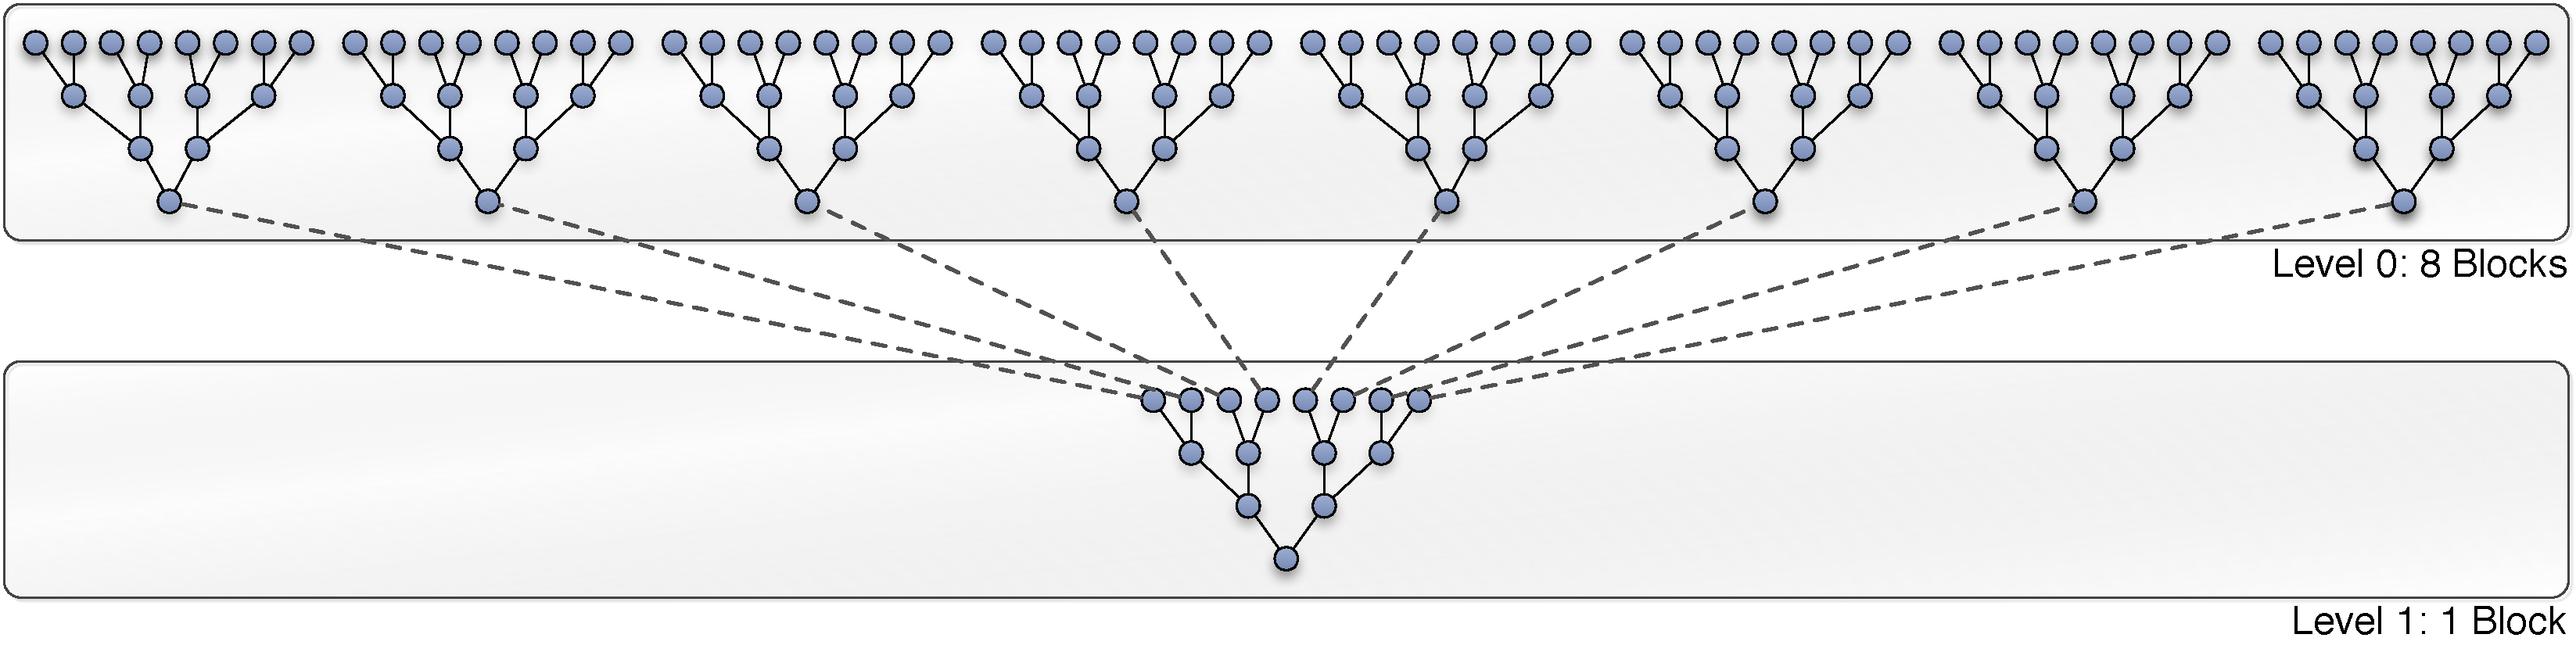
\includegraphics[width=\textwidth]{images/sec-4/tree-reduction}
    \end{center}
    \caption[A parallel tree reduction]{Illustration of a tree reduction,
        performed in two steps. In the first step 8 thread blocks in parallel
        reduce eight segments of the array to a single element each. The thread
        blocks synchronise by writing their result to memory, and the kernel is
    called recursively until the final scalar result is computed.}
    \label{fig:tree_reduction}
\end{figure}

If we wish to fuse other operations into the fold kernel, such as an element
wise multiplication from a dot product operation (\S\ref{sec:dotp}), only the
first line of reductions at level zero perform the element wise multiplication.
All subsequent reductions in that kernel, as well as the recursive steps at
level one and beyond, are pure reductions. Thus, the fused operation requires
compilation of two separate kernels. % We focus on the level zero kernel, which
is more interesting.

\subsubsection{Parallel Reduction Complexity}
\label{sec:parallel_reduction_complexity}

If each thread combines two elements at a time, then a vector of length $N$ will
\marginnote{tk: for non power-of-2 n, add upper/lower bounds symbols}
be reduced in $\mathcal{O}\left( \log N \right)$ parallel steps. Each step $S$
does $\sfrac{N}{S^2}$ independent operations, so the \emph{step
complexity}\index{complexity!step} of the algorithm is:
\[
\mathcal{O}\left( \log N \right)
\]
For $N=2^{D}$, the algorithm thus performs $\sum_{S=1}^{D}2^{D-S} = N - 1$
operations. This means that the \emph{work complexity}\index{complexity!work} of
the algorithm is:
\[
\mathcal{O}\left( N \right)
\]
and so does not perform more work than a sequential algorithm. For $P$ threads
running physically in parallel on $P$ processors, the \emph{time
complexity}\index{complexity!time} is $\mathcal{O}\left( \sfrac{N}{P} + \log N
\right)$. In a thread block $N = P$, so the time complexity is:
\[
\mathcal{O}\left( \log N \right)
\]
Compare this to a sequential reduction, which has a time complexity of
$\mathcal{O}\left( N \right)$.

\subsubsection{Algorithm Cascading}
\label{sec:algorithm_cascading}

The \emph{cost} of a parallel algorithm is the number of processors $\times$
time complexity. This implies that the cost of the algorithm is
$\mathcal{O}\left( N \log N \right)$, which is \emph{not} cost efficient.

Brent's theorem~\cite{Chatterjee:2009vh} suggests that instead of each thread
summing two elements, \emph{algorithm cascading} can be used to combine a
sequential and parallel reduction. Each thread does $\mathcal{O}\left( \log N
\right)$ sequential work, which reduces the cost of the algorithm to
$\mathcal{O}\left( \sfrac{N}{\log N} \log N \right)$, or rather:
\[
\mathcal{O}\left( N \right)
\]
while keeping the work complexity $\mathcal{O}\left( N \right)$ and step
complexity $\mathcal{O}\left( \log N \right)$.

This suggests, for example, that a block of 256 threads should sum a total of
2048 elements. In practice it is beneficial to do even more sequential work per
thread, since this reduces the number of levels in the recursive tree reduction
and provides better latency hiding.


\subsubsection{Mapping to CUDA Threads}

Reduction of a one dimensional array uses multiple thread blocks to
cooperatively reduce the array, as described above. The number of thread blocks
is limited to the maximum number of blocks that can be simultaneously resident
on the current device, which requires that blocks each do a larger amount of
sequential work before beginning the cooperative reduction phase. This limits
the total kernel startup cost associated with launching thread blocks. Since the
maximum number of resident blocks is typically much less than the number of
threads in a block, the reduction will typically require at most two kernel
invocations.\footnote{Accelerate selects the thread block size in order to
maximise thread occupancy. As this depends on both the specific \GPU being used
as well as the user function the array is reduced with, an upper bound of two
parallel steps can not be guaranteed.}

Higher-dimensional reductions reduce the array along the innermost dimension
only. This is similar to a segmented fold, except that the segment descriptor is
not necessary since the length of every segment is the same and can be
determined from the array shape. Instead of thread blocks cooperatively reducing
each segment sequentially, each segment is reduced by a single thread block
which operates independently of all other thread blocks. A consequence of this
is that proper device utilisation depends on the shape of the array and not
simply the total number of elements in the array. For example, reduction of an
array with shape @(Z :. 1 :. n)@ will use a single thread block, no matter
how large @n@ is. This simplifies the implementation but is clearly not
always ideal.\footnote{The number of multiprocessors on a device various between
architecture generation and performance of a given card. For example, a Tesla
T10 processor (compute compatability 1.3) has 240 cores split over 30
multiprocessors, while a Kepler K20X processor (compute capability 3.5) has 2688
cores split over only 14 multiprocessors. A given architecture generation will
have the same number of cores per multiprocessor, and lower performance
processors in a generation are produced by incorporating (or activating) fewer
multiprocessors, thereby reducing the total core count.}

A segmented reduction uses a single warp to reduce each segment. Investigation
of whether it is be better to convert the multidimensional reduction to a warp
per segment strategy, rather than mapping one thread block per segment as is
done currently, is left for future work.


\subsection{Scan}

Parallel scan and segmented scan algorithms are a crucial building block for a
great many data-parallel algorithms~\cite{Blelloch:1990ts,Chatterjee:1990vj}.
They also form the basis for efficiently mapping nested data-parallel languages
such as NESL~\cite{Blelloch:1995ut,Blelloch:1996jx} on to flat data-parallel
machines. Because of their fundamental importance to many algorithms,
implementing efficient scan operations in \CUDA has received much
attention~\cite{Sengupta:2007tc,Dotsenko:2008fo,Harris:2012fy}.

TK: A basic description (in pictures) of how the scan and segmented scan
algorithms work.


\subsection{Permute}

The @permute@ collective operation defines a forward permutation $f$ as an
index mapping from one array $X$ onto the result array $Y$, which we can write
as  $f : X \rightarrow Y$. Implementation of the permute function in Accelerate
is complicated because we have not placed any particular restrictions on $f$,
namely:
%
\begin{enumerate}
    \item $f$ is not surjective: the range of $f$ may not cover the codomain
        $Y$. For every $x$ in $X$, $f\left( x \right)$ need not yield every
        index $y$ in $Y$. This means that the result array must first be
        initialised with a set of default values.

    \item $f$ is not injective: distinct elements of the domain may
        map to the same element in the codomain. For all $x$ and $x'$ in $X$, if
        $f\left( x \right) = f\left( x' \right)$, we may have that $x \ne x'$.
        This means we require an associative combination function to combine
        elements from the domain that map to the same index in the codomain.

    \item $f$ is partial: elements of the domain may be ignored, and thus do
        not map to elements in the codomain.
\end{enumerate}

That the permutation function admits partial functions in the index mapping is
not particularly challenges for the implementation, and indeed is useful for
implementing the @filter@ operation, shown in Listing~\ref{lst:filter}. The
special value @ignore@ is used to drop elements of the input vector that do
not satisfy the predicate, by not mapping those indices to an index in the
codomain.
%
\begin{lstlisting}[style=haskell
    ,label=lst:filter
    ,caption={[Filter in Accelerate] Filtering returns only those elements of a
    vector which satisfy a predicate. This operation is included as part of
    Accelerate's standard prelude.}]
filter :: Elt a => (Exp a -> Exp Bool) -> Acc (Vector a) -> Acc (Vector a)
filter p vec
  = let flags            = map (boolToInt . p) vec
        (targetIdx, len) = scanl' (+) 0 flags
        defaults         = backpermute (index1 $ the len) id vec
    in
    permute const defaults (\ix -> flags!ix ==* 0 ? (ignore, index1 $ targetIdx!ix)) vec
\end{lstlisting}

On the other hand, because we can not prove that @filter@ is surjective, we
require the result vector to be first initialised with default values. Since we
do not know anything about the element type @a@, the only recourse is to
copy elements from the input array @vec@. This is doubly wasteful, because
we must first execute the @backpermute@ kernel to compute the
@defaults@ array, and then copy those values into the results vector before
executing the @permute@ kernel, even though we know the initialised values
will be completely overwritten.

At a second example, Listing~\ref{lst:histogram} demonstrates the computation of
a simple ten bin histogram from a vector of floating point elements in the range
$\left[ 0, 100 \right)$. In this case the permutation function is neither
surjective nor injective, as some bins may contain no elements and thus take the
default value, while other bins may contain multiple elements which need to be
combined (accumulated) correctly.
%
\begin{lstlisting}[style=haskell
    ,label=lst:histogram
    ,caption={[Simple histogram in Accelerate] A simple histogram written in
    Accelerate. We assume the input vector contains elements in the range
    $\left[0,100\right)$ and accumulate into ten equally sized bins.}]
histogram :: Acc (Vector Float) -> Acc (Vector Int)
histogram vec
  = let bins      = 10
        zeros     = fill (constant (Z :. bins)) 0
        ones      = fill (shape vec)            1
    in
    permute (+) zeros (\ix -> index1 (A.floor ((vec ! ix) / P.fromIntegral bins))) ones
\end{lstlisting}

The semantics of the operation is that every permutation from source to result
array is applied at the same time in a single parallel step. If multiple \CUDA
threads attempt a non-atomic write to the same memory location at the same time,
the writes will be serialised but the thread which performs the final write is
undefined, and so the final value at that memory slot is also
undefined~\cite{NVIDIA:2012wf}. To support non-injective permutation functions,
which are required to evaluate the histogram program correctly, the atomic
compare-and-swap operation is used to implement write combining.\footnote{The
atomic compare-and-swap operation on 32-bit values into global memory is only
available for devices of compute capability 1.1 and higher, and for 64-bit
values on devices of compute capability 1.2 and higher.} For a combination
function @f@ on elements of type @T@, the following atomically combines a value
from the source array @x@ with the value of the result array @y@.

\begin{lstlisting}[style=cuda]
    T x         = source[i];
    T y, old_y  = result[j];
    do {
        y       = old_y;
        old_y   = atomicCAS(&result[j], y, f x y);
    } while (y != old_y);
\end{lstlisting}
%
Any atomic operation on simple types can be implemented in terms of
compare-and-swap in this manner. Types consisting of more than one primitive
type, such as tuples, apply the procedure to each component separately.
Utilising more specific atomic operations such as @atomicAdd@ when
available is left to future work.

\subsection{Stencil}

TK: stencil


\section{Embedding GPU programs as skeletons}
\label{sec:code_generation}

Accelerate offers a range of aggregate operations on multi-dimensional arrays.
They include operations modelled after Haskell's list library, such as
@map@ and @fold@, but also array-oriented operations, such as
@permute@ and stencil convolutions.

As a simple example, consider the dot product of two vectors:
%
\begin{lstlisting}[style=haskell]
dotp :: Acc (Vector Float) -> Acc (Vector Float) -> Acc (Scalar Float)
dotp xs ys = fold (+) 0 (zipWith (*) xs ys)
\end{lstlisting}
%
The crucial difference to vanilla Haskell is the @Acc@ type constructor
representing \emph{embedded array-valued computations}. The types
@Vector e@ and @Scalar e@ represent one-dimensional and
zero-dimensional (singleton) arrays, respectively.

The expression @zipwith (*) xs ys@ implements point-wise multiplication of
the two argument vectors, and @fold (+) 0@ sums the resulting products up
to yield the final, scalar result, wrapped into a singleton array. The type of
@fold@ is:
%
\begin{lstlisting}[style=haskell]
fold :: (Shape sh, Elt a)
     => (Exp a -> Exp a -> Exp a)
     -> Exp a
     -> Acc (Array (sh:.Int) a)
     -> Acc (Array sh a)
\end{lstlisting}
%
It uses a binary folding function operating on \emph{embedded scalar
computations} of type @Exp a@ to implement a parallel reduction along the
innermost dimension of an $n$-dimensional, embedded array of type \code{Array
(sh:.Int) a}. The \emph{shape} @sh:.Int@ consist of a polymorphic shape
@sh@ with one added (innermost) dimension, which is missing from the shape
of the result array.


\subsection{Array operations as skeletons}

The Accelerate \CUDA backend is based on the idea of \emph{algorithmic
skeletons}~\cite{Cole:1989vr}, where a parallel program is composed from one or
more parameterised skeletons, or templates, encapsulating specific parallel
behaviour. In our case, the backend implements each of the aggregate array
operations, such as @map@, by way of a CUDA C \emph{code template} that is
parameterised with array types and worker functions, such as the function to be
mapped, to be injected at predefined points.

This generative approach is attractive for specialised hardware, such as GPUs,
as the code templates can be hand-tuned to avoid expensive control flow, ensure
efficient global-memory access, and use fast on-chip shared memory for local
communication --- all of which is necessary to ensure good performance on the
\GPU~\cite{NVIDIA:2012wf}.

In the first version of Accelerate, we implemented CUDA C code templates and
template instantiation with a mixture of C++ templates and C preprocessor
macros, which was described in \cite{Chakravarty:2011fr}. While workable, this
approach turned out to have a number of problems:

\begin{itemize}
    \item The use of CPP is fragile and difficult to maintain. Template
        instantiation by inlining of CPP macros required the use of fixed
        variables with no static checking to ensure the consistent use of names
        or that used names where defined before their use. Moreover it was easy
        to generate code that wasn't even syntactically valid.

    \item The approach led to the generation of dead code whenever specific
        template instances did not use all of their parameters or fields of
        structured data, which the CUDA compiler was unable to remove as dead
        code.

    \item Most importantly, the use of CPP did not scale to support the
        implementation of producer-consumer skeleton fusion, which is a crucial
        optimisation, even for code as simple as dot product.

\end{itemize}

The next sections discuss the new approach to template instantiation that avoids
these problems, and appeared in \cite{CliftonEverest:2014vi}.


\subsection{Algorithmic skeletons as template meta programs}

The code generator includes \CUDA code skeletons implementing each of the
collective operations in Accelerate. Each skeleton encodes the behaviour for
each thread for this collective operation, fixing the parallel algorithmic
structure of the operation. Each skeleton contains placeholders for the inputs
that parameterise the skeleton, such as the array types and worker functions.
Due to the shortcomings of C++ templates and CPP, we instead use Mainland's
\emph{quasiquotation} extensions~\cite{Mainland:2007bl} to Template
Haskell~\cite{Sheard:2002wu} to define skeletons as quoted \CUDA C templates
with splices for the template parameters.

Listing~\ref{lst:map_skeleton} shows the skeleton code for the @map@
operation. The @[cunit|...|]@ brackets enclose \CUDA C definitions
comprising this skeleton template. \CUDA uses the @__global__@ keyword to
indicate that @map@ is a \emph{GPU} \indexe{kernel}~\cite{NVIDIA:2012wf}
--- a single data-parallel computation launch on the \GPU by the CPU.
\emph{Antiquotations}\index{antiquotation} @$params:var@, @$exp:var@,
@$items:var@, and @$stms:var@ denote template parameters using a
Haskell variable @var@ to splice \CUDA C parameters, expressions, items,
and statements, respectively, into the skeleton.

\begin{lstlisting}[style=haskell,
    float,
    name=map_skeleton,
    label=lst:map_skeleton,
    caption={Accelerate CUDA skeleton for the @map@ operation}]
[cunit|
    $esc:("#include <accelerate_cuda.h>")
    $edecls:texIn

    extern "C" __global__ void
    map
    (
        $params:argIn,                                                                 -- (3)
        $params:argOut
    ){
        const int shapeSize     = size(shOut);
        const int gridSize      = $exp:(gridSize dev);
              int ix;

        for ( ix =  $exp:(threadIdx dev); ix < shapeSize; ix += gridSize )
        {
            $items:(dce x       .=. get ix)                                            -- (2)
            $items:(setOut "ix" .=. f x)                                               -- (1)
        }
    }
  |]
\end{lstlisting}

In order to instantiate the @map@ skeleton, the code generator needs to
generate concrete parameters for all of the holes in the skeleton template. In
particular:
%
\begin{enumerate}
\item The function @f@ which is applied to each individual array element;

\item The function @get@, which extracts the appropriate input array
    element for the array index @ix@; and finally

\item The types of the input and output array arguments are collected and
    spliced into @argIn@ and @argOut@, respectively.

\end{enumerate}
%
The meaning of the auxiliary combinators @get@, @setOut@, @dce@, and @(.=.)@
will be explained in the following sections.

As the quasiquoter @[cunit|...|]@ is executed at Haskell compile time,
syntactic errors in the quotations and antiquotations, as well as their
composition, are detected at compilation time. Thus, we can be sure that the
generated skeleton code will be syntactically correct if the backend compiles.
See \cite{Mainland:2007bl} for more information on quasiquoters.


\section{Instantiating skeletons}

Accelerate is an \emph{embedded} language, meaning that while we write programs
using Haskell syntax, we do not compile arbitrary Haskell programs directly to
\GPU machine code. Rather, an Accelerate program generates at program runtime an
\emph{abstract syntax tree} (\AST\index{AST|see{abstract syntax tree}}) that
represents the embedded program.
% We regard the collective array operations
% constituting the embedded program as algorithmic skeletons.
The job of Accelerate's CUDA backend code generator is to instantiate \CUDA
implementations of these collective operations, which are then compiled, loaded
onto the \GPU, and executed.

For the most part, translating Accelerate scalar expressions to plain \CUDA C
code is a straightforward syntactic translation of the \indext{de Bruijn} \AST
to C. The quasiquoting library \texttt{language-c-quote}%
\footnote{\url{http://hackage.haskell.org/package/language-c-quote}} allows the
\CUDA \AST to be constructed using concrete syntax. The following sections
describe some particular features of code generation.

% The following features of code generation deserve particular attention: lambda
% abstractions; let bindings; shapes; array references; and tuples.


\subsection{Producer-consumer fusion by template instantiation}
\label{sec:fusion_by_template_instantiation}

In the first, pre-template meta programming version of Accelerate based on C++
templates and CPP macros~\cite{Chakravarty:2011fr}, we generated one or more
CUDA GPU kernels for each aggregate array operation. This schema is undesirable
as it leads to many intermediate arrays and array traversals. Recall the
definition of vector dot product:
%
\begin{lstlisting}[style=haskell]
dotp :: Acc (Vector Float) -> Acc (Vector Float) -> Acc (Scalar Float)
dotp xs ys = fold (+) 0 (zipWith (*) xs ys)
\end{lstlisting}
%
The @zipWith@ and @fold@ operations would each compile to separate
skeletons, and as a result the execution of @zipWith@ produces an
intermediate array that the @fold@ kernels immediately consume.

This is not what a CUDA programmer would manually implement. It is more
efficient to inline the @zipWith@ computation into the kernel of the
@fold@. This strategy eliminates one GPU kernel, as well as one
intermediate array that is of the same extent as the [intersection of the] two
input arrays. To achieve the same performance as handwritten CUDA code, we
developed the short-cut fusion technique described in
chapter~\ref{ch:optimising}, and which appeared in \cite{McDonell:2013wi}.

The fusion system distinguishes producer-producer and consumer-producer fusion.
The former combines two skeletons where threads produce array elements
independently (such as @map@), from skeletons where threads cooperate to
produce an array (such as @fold@). Central to this approach is a
representation of arrays as functions, which we called \emph{delayed
arrays}\index{array!delayed} (in contrast to \emph{manifest
arrays}\index{array!manifest}) which are represented as follows:
%
\begin{lstlisting}[style=haskell]
  Delayed           :: (Shape sh, Elt e) =>
    { extentD       :: PreExp DelayedOpenAcc aenv sh            -- array extent
    , indexD        :: PreFun DelayedOpenAcc aenv (sh  -> e)    -- generate element at index\ldots
    , linearIndexD  :: PreFun DelayedOpenAcc aenv (Int -> e)    -- \ldots at linear index
    }               -> DelayedOpenAcc aenv (Array sh e)
\end{lstlisting}
%
Instead of generating a skeleton instance for @zipWith@ straight away, we
represent the computation implemented by @zipWith@ as a scalar function
(actually, a pair of functions) that generates an element of the array at a
given array index, together with the extent (domain) of the array, as a value of
type @DelayedOpenAcc@. For details of the representation see
section~\ref{sec:implementing_array_fusion}.

The crucial step in enabling producer-consumer fusion in Accelerate's CUDA
backend is in the function @codegenAcc@, which turns a manifest array
computation of type @DelayedOpenAcc aenv a@ into an instantiated CUDA
kernel of type @CUSkeleton aenv a@:
%
\begin{lstlisting}[style=haskell]
codegenAcc :: DeviceProperties
           -> DelayedOpenAcc aenv a
           -> Gamma aenv
           -> CUSkeleton aenv a
codegenAcc dev (Manifest pacc) aenv
  = case pacc of
      Fold f z a    -> mkFold dev aenv (codegenFun2 f) (codegenExp z) (codegenDelayed a)
      ...
\end{lstlisting}
%
Here we see that @mkFold@, which generates an instance of the @fold@
template, gets as its last argument the code generated for a delayed array
resulting from the call to @codegenDelayed@. The use of template meta
programming to implement CUDA skeletons is crucial to enable producer-consumer
fusion by way of template instantiation. In the dot product example, the delayed
producer is equivalent to the scalar function @\ix -> (xs!ix) * (ys!ix)@.
The call to @mkFold@ receives a CUDA version of this function, which can be
inlined directly into the @fold@ skeleton. The delayed producer function is
bound to the argument @getIn@ in the @mkFold@ definition given in
Listing~\ref{lst:mkfold}, which is used in the line marked \emph{(1)} and
expands to the following CUDA code:
%
\begin{lstlisting}[style=haskell]
const Int64 v1 = ({ assert(ix >= 0 && ix < min(shIn0_0, shIn1_0)); ix; });
y0 = arrIn0_0[v1] * arrIn1_0[v1];
\end{lstlisting}
%
Here the @assert@ checks whether the array index is in bounds, and is only
active when Accelerate is compiling kernels in debugging mode.\footnote{Kernel
debug mode is activated when the Accelerate CUDA backend is installed in debug
mode, and the command line flag \footcode{-ddebug-cc} is provided.} In this case the
embedded @zipWith@ operation is over two vectors, so no conversion to and
from multidimensional indices was required.

In contrast to the @map@ skeleton shown in Listing~\ref{lst:map_skeleton},
the code generated by @mkFold@ proceeds in to parallel phases. The first
phase is a sequential @for@ loop including the use of the @getIn@
embedded producer function. The second phase begins at the line marked
\emph{(2)} and implements a parallel tree reduction~\cite{Chatterjee:2009vh}.

\begin{lstlisting}[style=haskell
    ,float
    ,label=lst:mkfold
    ,caption={Accelerate CUDA skeleton for the @foldAll@ operation}]
mkFoldAll :: (Shape sh, Elt e)
          => DeviceProperties
          -> Gamma aenv
          -> CUFun2 aenv (e -> e -> e)
          -> CUExp  aenv e
          -> CUDelayedAcc aenv (sh :. Int) e
          -> CUTranslSkel aenv (Array sh e)
mkFoldAll dev aenv combine seed (CUDelayed shIn _ getIn)
  = CUSkeleton [cunit|

    $esc:("#include <accelerate_cuda.h>")
    $edecls:texIn

    extern "C" __global__ void
    foldAll
    (
        $params:argIn,
        $params:argOut
    )
    {
        // ommitted variable declarations

        $items:(sh .=. shIn)
        const int shapeSize     = $exp:(csize sh);
        const int gridSize      = $exp:(gridSize dev);
              int ix            = $exp:(threadIdx dev);

        if ( ix < shapeSize ) {
            $items:(y .=. getIn ix)

            for ( ix += gridSize; ix < shapeSize; ix += gridSize ) {
                $items:(x .=. getIn ix)                                                -- (1)
                $items:(y .=. combine x y)
            }
        }

        ix = min(shapeSize - blockIdx.x * blockDim.x, blockDim.x);
        $items:(sdata "threadIdx.x" .=. y)                                             -- (2)
        $items:(reduceBlock dev combine x y sdata ix)

        // first thread writes result to global memory
    }
  |]
\end{lstlisting}


\subsection{Instantiating skeletons with scalar code}
\label{sec:instantiating_skeletons}

Most aggregate array operations in Accelerate are parameterised by scalar
functions, such as the mapping function for @map@ or the combination
function for @fold@. Thus, a crucial part of template instantiation is
inlining \CUDA code implementing scalar Accelerate functions into the predefined
points of the template code. Inlining of scalar functions is always possible as
the scalar sub-language of Accelerate is first-order and does not support
recursion. These restrictions are necessary in order to generate \GPU code, as
\GPU hardware neither supports large stacks (for recursion) nor closures (for
higher-order functions).

To splice scalar code fragments into the skeleton code of array operations, we
define a typeclass of l-values and r-values to define a generic assignment
operator @(.=.)@. For example, the operator was used in lines \emph{(1)}
and \emph{(2)} of Listing~\ref{lst:map_skeleton}. This representation abstracts
over whether our skeleton uses l-values in single static assignment-style to
@const@ declarations, or as a statement updating a mutable variable. The
class declarations are the following:
%
\begin{lstlisting}[style=haskell]
class Lvalue a where
  lvalue :: a -> C.Exp -> C.BlockItem

class Rvalue a where
  rvalue :: a -> C.Exp

class Assign l r where
  (.=.) :: l -> r -> [C.BlockItem]

instance (Lvalue l, Rvalue r) => Assign l r where
  lhs .=. rhs = [ lvalue lhs (rvalue rhs) ]
\end{lstlisting}

Furthermore, we can also bring any additional terms into scope before evaluating
an r-value. For example, this instance is used to bring any let-bound terms into
scope before evaluating the body expression. We enable this by way of the
following class instance:
%
\begin{lstlisting}[style=haskell]
instance Assign l r => Assign l ([C.BlockItem], r) where
  lhs .=. (env, rhs) = env ++ assign lhs rhs
\end{lstlisting}


\subsection{Representing tuples}
\label{sec:representing_tuples}

Accelerate arrays of primitive type, such as @Float@ and @Int@, are
easily represented in CUDA using the corresponding floating point and integral
types. More interesting is the case of arrays of tuples. A na\"ive
implementation of tuples in CUDA might use arrays of @struct@ type --- that
is, we might consider representing values of type @Array DIM1 (Int, Float)@
in CUDA by the value of type:
%
\begin{lstlisting}[style=cuda]
typedef struct { int a; float b; } arrayIntFloat[];
\end{lstlisting}
%
Known as the \emph{array-of-struct} (\AoS\index{AoS|see {array-of-struct}})
representation, this strategy is in general not efficient as it easily violates
the strict memory access rules imposed on CUDA devices, decreasing effective
bandwidth by as much as an order of magnitude~\cite{NVIDIA:2012wf}.

\subsubsection{Non-parametric array representation}

To avoid this inefficiency, Accelerate uses a non-parametric array
representation: arrays of tuples are represented as tuples of arrays of
primitive type. This \emph{struct-of-array} (\SoA\index{SoA|see
{struct-of-array}}) representation stores arrays of type \code{Array DIM1 (Int,
Float)} by values of the type:
%
\begin{lstlisting}[style=cuda]
typedef struct { int a[]; float b[]; } arrayIntFloat;
\end{lstlisting}
%
By virtue of this non-parametric array representation, Accelerate (1) maintains
global memory access coalescing rules, and (2) is able to avoid redundant reads
of array elements that are never used. The second point will be discussed
further in the following section.

\subsubsection{Non-parametric scalar expressions}

This non-parametric array representation also existed in the old version of
Accelerate~\cite{Chakravarty:2011fr}. However, since code generation was based
on C++ templates and CPP macros, and moreover, the skeleton code was required to
abstract over array element types, C @struct@s were used to represent
tuples of scalar values. A family of getter and setter functions were then
generated to create and consume these @struct@s when reading and writing
elements of the non-parametric array representation.

However, this leads to the generation of dead code whenever specific template
instances don't use some of their parameters or fields of the structured data.
As an example, consider the following Accelerate function that projects the
first component of each element of a vector of quadruples:
%
\begin{lstlisting}[style=haskell]
fst4 :: Acc (Vector (a,b,c,d)) -> Acc (Vector a)
fst4 = map (\v -> let (x,_,_,_) = unlift v in x)
\end{lstlisting}
%
The function @unlift@ turns an embedded scalar expression that yields a
quadruple, into a quadruple comprising four embedded scalar expressions ---
hence, we can perform pattern matching in the let binding in order to unpack the
expression. Moreover, in @fst4@ under the old code generation strategy,
array elements are copied into a @struct@, only for the first element to be
extracted again and the @struct@ to be discarded. One might hope that the
\CUDA compiler (1) spots the redundant copying of array elements; and (2) that
the elements of three of the four arrays are never used. Alas, it does not, and
as a result @fst4@ generates considerable memory traffic.

With template meta programming and the @Assign@ type class introduced
previously, we fare much better. As the entire skeleton template is quasiquoted,
we can inline the definitions of scalar expressions, including array accesses,
directly into the skeleton template. Instead of packaging the tuple components
into a @struct@, we represent it by a list of primitive values, one per
component. During code generation, we keep track of the values constituting a
tuple by maintaining a list of expressions, one for each component of the tuple.
The @(.=.)@ operator allows us to assign all values constituting the tuple
with one assignment in the meta programming system; i.e., we have lists of
l-values and r-values:
%
\begin{lstlisting}[style=haskell]
instance Assign l r => Assign [l] [r] where
  []     .=. []     = []
  (x:xs) .=. (y:ys) = assign x y ++ assign xs ys
\end{lstlisting}


\subsection{Shared subexpressions}
\label{sec:shared_subexpressions}

A well known problem with deeply embedded languages is the issue of
\emph{sharing}, where --- without \emph{sharing recovery} --- each occurrence of
a let-bound variable in the source program creates a separate unfolding of the
bound expression in the reified program. To avoid this problem, we implemented a
sharing recovery algorithm that recovers exactly those let-bindings used in the
source language. See section~\ref{sec:sharing_recovery} for details on our
approach to sharing recovery~\cite{McDonell:2013wi}, which is a variant of
Gill's observable sharing~\cite{Gill:2009dx} --- his paper also discusses the
issue of sharing in embedded languages in greater detail.

Following sharing recovery and conversion of the source language program into
the internal \indext{de Bruijn} representation, sharing of scalar
subcomputations is represented explicitly using the following \AST node:
%
\begin{lstlisting}[style=haskell]
  Let :: (Elt bnd, Elt body)
      => PreOpenExp acc env        aenv bnd         -- (1) bound expression
      -> PreOpenExp acc (env, bnd) aenv body        -- (2) body expression, scope of local binding
      -> PreOpenExp acc env        aenv body
\end{lstlisting}
%
Here, the result of evaluating the let-bound expression (1) is only in scope
while evaluating the body of the let-binding (2). This property is encoded in
the type of the environment of the body expression.

To support code generation including shared subexpressions, the CUDA code
generator uses a monad to generate fresh names. The monad is also used to store
the expressions representing let-bound terms. These additional terms must be
evaluated before evaluation of the body.
%
\begin{lstlisting}[style=haskell]
data Gen = Gen
  { unique          :: Int
  , localBindings   :: [C.BlockItem]
  , usedTerms       :: Set C.Exp                    -- see section~\ref{sec:eliminating_dead_code}
  }
\end{lstlisting}

When code generation encounters a let binding, we first generate code for the
bound expression, assign this result to a new (fresh) variable, then use this
stored variable throughout the evaluation of the body:
%
\begin{lstlisting}[style=haskell]
codegenOpenExp (Let bnd body) env = do
    bnd'  <- codegenOpenExp bnd env >>= pushEnv bnd
    body' <- codegenOpenExp body (env `Push` bnd')
    return body'
\end{lstlisting}

Recall that Accelerate's \CUDA code generator uses a non-parametric
representation of tuples, where a scalar expression is represented as a list of
C expressions, one per component of the (flattened) tuple
(\S\ref{sec:representing_tuples}). The function @pushEnv@ generates a fresh
name for each expression in the tuple, assigns the expression to a new variable,
and returns the new variable name to be used throughout evaluation of the body
expression.
%
\begin{lstlisting}[style=haskell]
pushEnv :: exp env aenv a -> [C.Exp] -> Gen [C.Exp]
pushEnv dummy exps = zipWithM go (expType dummy) exps
  where
    go t c = case c of
      C.Var{}   -> return c
      _         -> do name    <- fresh
                      let next = [citem| const $ty:t $id:name = $exp:c; |]
                      modify (\s -> s { localBindings = next : localBindings s })
                      return (cvar name)
\end{lstlisting}
%
Note that there is no need to create a fresh name if the input term is a
variable. That is, we avoid creating additional declarations in the generated
code such as:
%
\begin{lstlisting}[language=cuda]
  const int x0 = ...
  const int x1 = x0;
\end{lstlisting}
%
This observation also simplifies the implementation of dead-code analysis
(\S\ref{sec:eliminating_dead_code}). The output of code generation is the list
of C expressions representing the final computation, together with a list of
local declarations to be evaluated first. With the @Assign@ type class
introduced previously, we can transparently bring these extra terms into scope
before evaluating the body, with the introduction of the following instance:
%
\begin{lstlisting}[style=haskell]
instance Assign l r => Assign l ([C.BlockItem], r) where
  lhs .=. (env, rhs) = env ++ (lhs .=. rhs)
\end{lstlisting}


\subsubsection{Future work}

One disadvantage of the current implementation is that the scope of let bindings
is lost: once a new variable is declared, it remains in scope for the remainder
of the C skeleton. This is in contrast to the definition of the @Let@ \AST
node, where the binding should only be in scope during evaluation of the body.
Adding explicit scoping to specify the lifetime of expressions may assist the
CUDA compiler to improve register allocation.

% Without adding explicit scoping to specify the lifetime of expressions, we
% rely on the CUDA compiler to efficiently allocate reg

Generating code with explicit scoping may also remove the need for a monad to
generate fresh names, since unique names can be derived based on the \indext{de
Bruijn} \emph{level} of the expression, which can be determined from the current
size of the environment. This is the method used when pretty printing Accelerate
expressions.


\subsection{Eliminating dead code}
\label{sec:eliminating_dead_code}

As discussed in section~\ref{sec:representing_tuples}, one problem of the
original code generator based on CPP and C++ templates was its inability to
remove some forms of dead code. This was seen in the @fst4@ example of
section~\ref{sec:representing_tuples}, which generates significant memory
traffic if tuples are represented as @struct@s, even though three of the
four values read from memory were never used. With the use of template meta
programming to inline the definition of scalar expressions directly into the
skeleton template, the situation is greatly improved.

Unfortunately, the CUDA compiler does not always eliminate memory reads, as it
does not always detect if the values are used. Hence, rather than rely on the
CUDA compiler, the code generation process explicitly tracks which values are
used at all in the generated scalar code, and when splicing assignments into a
skeleton template, we elide statements whose results are not used. The following
instance of the @Assign@ class uses a flag that is @False@ to indicate
that the assigned value is not used.
%
\begin{lstlisting}[style=haskell]
instance Assign l r => Assign (Bool,l) r where
  (used,lhs) .=. rhs
    | used      = assign lhs rhs
    | otherwise = []
\end{lstlisting}

The @map@ skeleton of Listing~\ref{lst:map_skeleton} exploits this: when
generating code for the mapped function @f@, the function \code{dce :: [a]
-> [(Bool,a)]} on the line marked \emph{(2)} is also generated, and determines
for each term whether it is subsequently used. Thus, when the code generated by
@get@ reads data from the input array, it doesn't read the unused values.
Consequently, @fst4@ only touches the array representing the first
component of the quadruple of arrays.

To generate the function @dce@ we need to determine which inputs to the
generated scalar function are ultimately used in the calculation. Code
generation for a function such as @fst4@ begins by initialising the
scalar environment of the function body with input variables of a known name
(1):
%
\begin{lstlisting}[style=haskell]
codegenFun1
    :: DeviceProperties
    -> Gamma aenv
    -> DelayedFun aenv (a -> b)
    -> CUFun1     aenv (a -> b)
codegenFun1 dev aenv (Lam (Body f))
  = let
        dummy        = locals "undefined_x" (undefined :: a)                        -- (1)
        Gen _ _ used = execGen $ codegenOpenExp dev aenv f (Empty `Push` dummy)     -- (2)
    ...
\end{lstlisting}
%
During code generation we build a set containing the variables that are used in
the function body. In (2) code generation proceeds with the dummy variables,
with the final state returned, which contains the set of used variables.
Dead-code analysis then builds the function @dce@ by testing whether each
input variable is present in the set:
%
\begin{lstlisting}[style=haskell]
deadCodeElim :: Set C.Exp -> [C.Exp] -> [a] -> [(Bool,a)]
deadCodeElim used vars
  = let flags = map (\x -> x `Set.member` used) vars
    in  zipWith (,) flags
\end{lstlisting}

During code generation, we must decide when to add variables to the set. In
general, we check the result from each step of @codegenOpenExp@ with the
function @visit@, and test if the result was a scalar C variable:
%
\begin{lstlisting}[style=haskell]
visit :: [C.Exp] -> Gen [C.Exp]
visit exp
  | [x] <- exp  = markAsUsed x >> return exp
  | otherwise   =                 return exp

markAsUsed :: C.Exp -> Gen ()
markAsUsed x@C.Exp{} = modify (\s -> s { usedTerms = Set.insert x (usedTerms s)} )
markAsUsed _         = return ()
\end{lstlisting}


\subsubsection{Future work}

Completing our definition of @codegenFun1@, we return the result of
dead-code analysis produced by @deadCodeElim@, together with a function
that \emph{re-runs} code generation with the actual input variables. Thus, our
method requires performing code generation at least twice for every expression:
once to generates usage information, and then again each time the function is
instantiated with a particular set of variables.
%
\begin{lstlisting}[style=haskell,firstnumber=7]
codegenFun1 dev aenv (Lam (Body f))
  = let
        dummy        = ...
        Gen _ _ used = execGen $ codegenOpenExp ...
    in
    CUFun1 (deadCodeElim used dummy)
           (\xs -> evalGen $ codegenOpenExp dev aenv f (Empty `Push` xs))
\end{lstlisting}

Furthermore, this method only eliminates unused inputs to a scalar function. If
the generated code produced intermediate values
(\S\ref{sec:shared_subexpressions}) based on these unused inputs, these
expressions will still appear in the generated code. We leave addressing both of
these issues to future work.


\subsection{Shapes and indices}

Parallelism in Accelerate takes the form of collective operations on arrays of
type @Array sh e@, where @sh@ is the \emph{shape} and \emph{e} is the
element type of the array. Following the approach taken in
Repa~\cite{Keller:2010er,Lippmeier:2012gx}, we represent both the shape and
indices of an array using an inductive notation of tuples as heterogenous
\emph{snoc} lists to enable rank-polymorphic definitions of array functions.

As shown in Listing~\ref{lst:shapes_and_indices}, on both the type and value
level, the constructor @Z@ is used to represent the shape of a rank-0
array, and the infix operator @(:.)@ to increase the rank by adding a new
(innermost) dimension to the right of the shape.

\begin{lstlisting}[style=haskell
    ,float
    ,label=lst:shapes_and_indices
    ,caption={Types of array shapes and indices}]
data Z            = Z                   -- rank zero
data tail :. head = tail :. head        -- increase rank by one

type DIM0 = Z
type DIM1 = DIM0 :. Int
type DIM2 = DIM1 :. Int
type DIM3 = DIM2 :. Int
  %$\langle$ and so on $\rangle$%

type Array DIM0 e = Scalar e
type Array DIM1 e = Vector e
\end{lstlisting}

During code generation, the old version of Accelerate~\cite{Chakravarty:2011fr}
represented multidimensional shapes and indices as a @struct@.
%
% \begin{lstlisting}[style=cuda]
% typedef Int32                           Ix;
% typedef void*                           DIM0;
% typedef struct { Ix a0; }               DIM1;
% typedef struct { Ix a1,a0; }            DIM2;
% typedef struct { Ix a2,a1,a0; }         DIM3;
%   (@*$\langle$ and so on $\rangle$*@)
% \end{lstlisting}
%
This representation additionally came with a family of overloaded C functions
for operating on shapes and indices --- such as @toIndex@ and
@fromIndex@ --- so that skeletons were not specialised to a particular
dimensionality.
%
% \begin{lstlisting}[style=cuda,mathescape]
% int  dim(DIM$n$ sh);                        // number of dimensions in a shape
% int  size(DIM$n$ sh);                       // total number of elements in a shape
% Ix   toIndex(DIM$n$ sh, DIM$n$ ix);            // index into a linear row-major format array
% DIM$n$ fromIndex(DIM$n$ sh, Ix ix);            // inverse of `toIndex'
% \end{lstlisting}

The new code generation method\footnote{Subsequent to, but not affecting the
result of \cite{CliftonEverest:2014vi}} does not require the use of @struct@s to
represent shapes. The new approach represents shapes during code generation in
the same manner as tuples --- as a list of expressions representing each of the
individual components of the shape. Operations such as @toIndex@ are implemented
directly in the skeleton, rather than packing the shape components into a
@struct@ and then calling the family of overloaded functions which were provided
separately in a header file.

Recall the vector dot product example from
section~\ref{sec:fusion_by_template_instantiation}, where the pairwise
multiplication of the two arrays resulting in the scalar function
@\ix -> (xs!ix) * (ys!ix)@ being embedded into the consumer template. If a
@struct@-based representation of shapes is used, this results in the following
C code~\cite{CliftonEverest:2014vi}:
%
\begin{lstlisting}[style=cuda]
  const Int64 v2 = ix;
  const int v3 = toIndex(shIn0, shape(v2));
  const int v4 = toIndex(shIn1, shape(v2));
  y0 = arrIn0_a0[v3] * arrIn1_a0[v4];
\end{lstlisting}
%
The functions @shape@ and @toIndex@ map multi-dimensional indices to the linear
array representation. Since the source arrays are vectors, they do not
contribute anything to the example, in particular, their definitions are:
%
\begin{lstlisting}[style=cuda]
static __inline__ __device__ int toIndex(const DIM1 sh, const DIM1 ix)
{
    assert(ix >= 0 && ix < sh);
    return ix;
}

static __inline__ __device__ DIM1 shape(const int a)
{
    return a;
}
\end{lstlisting}
%
Thus, @v3@ and @v4@ map, indirectly, to @v2@ and --- luckily --- the CUDA
compiler is able to remove the superfluous assignments in this case. With the
new code generator method, we produce the following code which does not
introduce the redundant assignment, and thus does not rely on optimisations
performed by the CUDA compiler:
%
\begin{lstlisting}[style=cuda]
const Int64 v1 = ({ assert(ix ≥ 0 && ix < min(shIn0_0, shIn1_0)); ix; });
y0 = arrIn0_0[v1] * arrIn1_0[v1];
\end{lstlisting}


\subsection{Lambda abstractions}

Concerning lambda abstractions, we mentioned previously that Accelerate's scalar
expression language is first order, in the sense that, although it includes
lambda abstractions, it does not include a general application form. This
ensures that lambda abstractions of scalar expressions can only be used as the
arguments to collective operations, such as @zipWith@. This restriction is
necessary in order to generate code for \GPU hardware. As a consequence, lambda
abstractions are always outermost (in type correct programs) and we can always
translate them into either (a) plain C functions, or (b) inline them directly
into the use site. The old code generator had no choice but to select the first
alternative, whereas the new method can make use of several optimisations by
using the second, such as def-use analysis (\S\ref{sec:eliminating_dead_code}).

A recent change to the array and scalar language has been the introduction of
explicit value iteration. In the scalar language, this is encoded with the
following \AST node, which behaves analogously to a standard C while loop:
%
\begin{lstlisting}[style=haskell]
While :: Elt a
      => PreOpenFun acc env aenv (a -> Bool)    -- (1) continue while true
      -> PreOpenFun acc env aenv (a -> a)       -- (2) function to iterate
      -> PreOpenExp acc env aenv a              -- initial value
      -> PreOpenExp acc env aenv a
\end{lstlisting}
%
Although we use scalar functions to represent the iteration test (1) and loop
body (2), the operation is suitably restricted so that, so long as some care is
taken when generating C code for the loop, we do not need to perform lambda
lifting of the function valued arguments. However, we can not use the standard
@codegenFun1@ operation to generate the CUDA code for the unary function,
as this unfortunately interferes with our implementation of def-use analysis
(\S\ref{sec:eliminating_dead_code}).

The following function is used to generate C code for the loop operations, which
generates code for the function body in a clean environment (1), and restores
the outer environment on exit (2), including any newly introduced bindings as
part of the return value (3).
%
\begin{lstlisting}[style=haskell]
cvtF1 :: DelayedOpenExp env aenv t -> Val env -> Gen ([C.BlockItem], [C.Exp])
cvtF1 (Lam (Body e)) env = do
  old  <- state (\s -> ( localBindings s, s { localBindings = []  } ))              -- (1)
  e'   <- codegenOpenExp e env
  env' <- state (\s -> ( localBindings s, s { localBindings = old } ))              -- (2)
  return (reverse env', e')                                                         -- (3)
\end{lstlisting}
%
Thus, any shared subexpressions (\S\ref{sec:shared_subexpressions}) encountered
during code generation are evaluated before executing the function body, using
the @Assign@ class discussed earlier.


\subsection{Array references in scalar code}

Accelerate includes two scalar operations that receive an array-valued argument,
namely array indexing (@!@ and @!!@) and determining the @shape@
of an array. These are, for example, used in the sparse-matrix vector
multiplication operation shown in Listing~\ref{lst:smvm}. Specifically, this
code includes the following use of @backpermute@ to extract the values of
the vector that are to be multiplied with the non-zero elements of the sparse
matrix:
%
\begin{lstlisting}[style=haskell]
A.backpermute (shape inds) (\i -> index1 $ inds!i) vec
\end{lstlisting}
% \begin{lstlisting}[style=haskell]
% smvm :: Acc (SparseMatrix Float) -> Acc (Vector Float) -> Acc (Vector Float)
% smvm smat vec
%   = let (segd, svec)    = A.unlift smat
%         (inds, vals)    = A.unzip svec
%         vecVals         = A.backpermute (shape inds) (\i -> index1 $ inds!i) vec
%         products        = A.zipWith (*) vecVals vals
%     in
%     foldSeg (+) 0 products segd
% \end{lstlisting}
%
Here the array computation @inds :: Acc (Array DIM1 Float)@ is used in the
first and second argument of @backpermute@. In the code for @smvm@,
@inds@ is a previously let-bound variable. If instead, a collective
operation would have been used in place of @inds@ in the scalar function
@\i -> index1 $ inds!i@, we would lift it out of the scalar function and
let bind it. After all, we do not want to execute an arbitrarily complex array
computation once for every invocation of a scalar function. In fact, CUDA does
not permit us to do this, as the scalar function is translated into GPU kernel
code, and kernel code can not include further nested parallelism.

Nevertheless, even though array valued arguments to scalar functions will always
be let-bound variables, code generation is not straightforward. In the old
version of Accelerate~\cite{Chakravarty:2011fr}, generated code was not able to
add a new argument to the prototype of the @backpermute@ skeleton, as the
generated code simply included the skeleton definition using a C pre-processor
@include@ directive. This problem was worked around by using \emph{texture
references} --- a CUDA feature that comes from its graphics heritage --- to
define what are essentially read-only arrays as global tables on a per skeleton
instantiation basis. The use of texture references had another happy
consequence. Skeletons such as @backpermute@ allow unconstrained indexing
patters, which may not follow the strict requirements for coalesced and aligned
access to global memory, which can incur a severe performance
penalties~\cite{NVIDIA:2012wf}. However, texture memory access is cached, and
hence, may be more efficient in these circumstances.

In contrast to a traditional cache such as on a CPU, while the texture cache is
designed to reduce bandwidth requirements to global memory, it does not reduce
the access \emph{latency}~\cite[\S5.3.2]{NVIDIA:2012wf}. However, beginning with
Compute Capability 2.0, the GPU also comes equipped with a traditional L2 cache.
Since the new code generator based on quasiquoting~\cite{CliftonEverest:2014vi}
is are able to dynamically rewrite the entire skeleton --- in particular
including the function prototype --- we are no longer forced to access
array-valued arguments via the texture cache.

In order to use the inbuilt L2 cache available in devices of compute capability
2.0 and higher, arrays referenced from scalar code are marshalled to the kernel
via the kernel function parameters, and read via standard array indexing. For
older series 1.x devices that do not have a L2 cache, the texture cache is still
used instead.


\subsection{Conclusion}

The use of template meta programming for skeleton definition and instantiation
enables us to combine the advantages of conventional code generators (such as
def-use analysis for dead code elimination) with those of generative
skeleton-based code generators (such as handwritten idiomatic code for
special-purpose architectures).


\section{Dynamic compilation \& code memoisation}
\label{sec:dynamic_compilation}

When you write a program in Accelerate, what you are really doing is writing a
Haskell program that \emph{generates} a \CUDA program, that is compiled,
loaded, and executed on the \GPU\@. Thus, one major difference between using
Accelerate for general purpose \GPU programming compared to programming in
\CUDA directly, is that kernels are generated dynamically, at application
\emph{runtime}, whereas plain \CUDA code is pre-compiled.

Dynamic code generation has significant advantages, especially for embedded
languages. In particular, the code generator can query the capabilities of the
hardware on which the code will be executed, and optimise the generated program
accordingly, as well as specialise the code to the available input data. The
host program can also be used to generate the embedded program.

The main drawback of dynamically generating and compiling \GPU kernels is the
additional execution time required to do so, so attempts must be made to
mitigate these overheads. In general purpose \GPU programming, it is only
worthwhile to offload computations to the \GPU if they are computationally
intensive. This implies a significant runtime and usually also the use of
significant amount of input and/or output data. Hence, the overhead of dynamic
kernel compilation is not necessarily problematic in the face of long kernel
runtimes and long data-transfer times between host and device memory, especially
if those kernels are compiled once and executed on multiple data sets.

\subsection{External compilation}
\label{sec:external_compilation}

In unison with the \AST traversal that extracts @Use@ subterms to initiate
data transfers (\S\ref{sec:host_device_transfers}), the \CUDA backend initiates
code generation for each collective array operation it encounters via skeleton
instantiation (\S\ref{sec:code_generation}). After the \CUDA code is generated,
it must be compiled with the external \texttt{nvcc} tool-chain to produce binary
object code for the kernels implementing each collective operation.

As with data transfer, the compilation of the generated \CUDA code proceeds
asynchronously, and linking of the compiled code is deferred until it is needed
during execution. For each generated kernel, the \CUDA compiler is invoked by
spawning an external process that executes the raw system command. However, if
the program requires the compilation of many kernels, carelessly spawning a new
process for every instantiated skeleton can cause the IO bus to become
saturated, further increasing compilation time, or exhaust the host operating
system's available process handles. To counter this problem, a worker pool is
created that will be used to process jobs in first-in first-out (FIFO) order:
%
\begin{lstlisting}[style=haskell]
{-# NOINLINE worker #-}
worker :: Queue.MSem Int
worker = unsafePerformIO $ Queue.new =<< getNumProcessors
\end{lstlisting}

The worker pool is defined as the Haskell equivalent of a global
variable\footnote{The idiom popularly known as ``the unsafePerformIO hack''.}
and is initialised once per program execution. The number of slots in the queue
is set to the number of physical CPU cores present in the host
system\footnote{Note that this is not limited by the RTS option \texttt{-N} that
specifies the number of processors to use.} which specifies the maximum number
of kernels to compile concurrently. Instead of initiating the compilation
process directly, it is instead added to the work queue:
%
\begin{lstlisting}[style=haskell,firstnumber=last]
enqueueProcess :: FilePath -> [String] -> IO (MVar ())
enqueueProcess nvcc flags = do
  mvar  <- newEmptyMVar                                         -- (2)
  _     <- forkIO $ do                                          -- (1)
    Queue.with worker $ do                                      -- (3)
        (_,_,_,pid)     <- createProcess (proc nvcc flags)
        waitFor pid
    --
    putMVar mvar ()                                             -- (4)
  --
  return mvar
\end{lstlisting}

\begin{enumerate}
\item The process is spawned from a separate thread so that the thread can block
    waiting for both the worker queue and the external process, without
    interrupting the main thread. Thus compilation proceeds asynchronously with
    outer host processing tasks.

\item An empty @MVar@ is created that will act as a signal to the main
    thread that the external process has completed. Since @takeMVar@ on an
    empty @MVar@ blocks until that @MVar@ is filled, the main thread
    can wait for the external process to complete if the compiled code is not
    yet available by the time it is required during the execution phase.

\item The thread waits for a worker to become available from the queue. Blocked
    threads are woken up by the runtime system and are serviced in a first-in
    first-out order; that is, threads do not actively poll the queue continually
    testing for an open slot. Once a worker becomes available, the external
    process is launched and the thread once again blocks until that process
    completes.

\item Once the process completes the worker is returned to the queue where it
    can be assigned to handle any further tasks. Finally, the thread fills the
    @MVar@ to signal the main thread that the compilation has completed.
\end{enumerate}

We return to the question of linking in the compiled code below, when we discuss
the process of executing the program.


\subsection{Caching compiled kernels}
\label{sec:caching_compiled_kernels}

The \CUDA backend associates each \CUDA binary with the skeleton instantiation
whose computation that binary implements. Furthermore, the binary object code is
keyed on a skeleton and the parameters of its instantiation, not to the specific
AST node used to instantiate the skeleton. As a result, compiled binaries are
reusable when the same skeleton instantiation is required again, whether that is
in the same Accelerate computation applied to a different set of input arrays,
or an entirely different computation. For example, operations such as
@scanl (+) 0@ are common, and it would be wasteful to dynamically generate
and compile the same code multiple times.

\begin{lstlisting}[style=haskell,numbers=none]
type ProgramCache = HashTable KernelKey KernelEntry

type KernelKey = (CUDA.Compute, ByteString)
data KernelEntry
    = CompileProcess FilePath (MVar ())                                 -- (1)
    | KernelObject ByteString (FullList CUDA.Context CUDA.Module)       -- (2)
\end{lstlisting}

The cache is a hash table which is keyed by an MD5~\cite{Rivest:1992va} digest
of the generated \CUDA code which instantiates the skeleton, as well as the
compute capability the generated code was specialised and compiled for. The hash
table value can either refer to:
%
\begin{enumerate}
\item A currently compiling external process. This records the path of the file
    currently being compiled, which will be rooted in a temporary directory, as
    well as the @MVar@ that will signal when the external process has
    completed (\S\ref{sec:external_compilation}). If a kernel is requested that
    is currently compiling, the thread blocks on the @MVar@ until the
    result is available and then updates the hash table with;

\item The raw compiled data with a non-empty list of \CUDA contexts that the
    object code has been linked into. The entry may have been added to the cache
    by an alternate context of the same compute capability, for example on a
    system with multiple \CUDA devices, so the code simply needs to be
    re-linked for the current context.
\end{enumerate}

This scheme effectively caches kernels both within the same Accelerate
computation and across different Accelerate expressions. However, it must be
regenerated ever time the program is executed, which increases program startup
time. Once a kernel is compiled, the binary object code is saved in the user's
home directory so that it is available across separate runs of the program, or
indeed different programs. This information is stored in a persistent cache:
%
\begin{lstlisting}[style=haskell,numbers=none]
type PersistentCache = HashTable KernelKey ()
\end{lstlisting}

The persistent cache is a hash table indexed by the same key used by the
in-memory cache described above, but without a value component. Instead, the
presence of a key in the persistent cache indicates that the compiled binary
represented by that key is available to be loaded from disk. The location of the
object code is determined from the MD5 digest by creating a ASCII representation
of the digest, replacing special characters with z-encoded strings.
%
\begin{lstlisting}[style=haskell]
encode_ch :: Char -> String
encode_ch c | unencodedChar c = [c]             -- regular characters except `z' and `Z'
encode_ch '('  = "ZL"                           -- punctuation using two-character sequences
encode_ch ')'  = "ZR"
  ...
encode_ch c    = encode_as_unicode_char c       -- other characters using hexadecimal
\end{lstlisting}

Initialising the persistent cache populates the hash table by reading an index
file from disk, which is simply a binary file containing the number of entries
at the start of the file, followed by the keys.
%
\begin{lstlisting}[style=haskell]
restore :: FilePath -> IO PersistentCache
restore db = do
  exist <- doesFileExist db
  case exist of
    False       -> encodeFile db (0::Int) >> HashTable.new
    True        -> do
      store         <- L.readFile db
      let (n,rest,_) = runGetState get store 0
      pt            <- HashTable.newSized n
      --
      let go []      = return ()
          go (!k:xs) = HashTable.insert pt k () >> go xs
      --
      go (runGet (getMany n) rest)
\end{lstlisting}

The \texttt{binary} package is used to deserialise the data from file. Note that
the implementation for serialising lists of elements provided by that preserves
the order of elements in the list, which requires creating the entire list
structure in memory.\footnote{A tail-recursive loop that accumulates the list
structure as the file is read sequentially from disk produces list elements in
reverse order. Thus, the list must be reversed before being returned, making the
structure spine-strict and preventing elements being consumed as they are read
from file.} Since we do not require this property, we provide our own
deserialisation routine that allows the elements to be lazily consumed and added
directly to the hash table as they are read from file.

\begin{lstlisting}[style=haskell]
getMany :: Binary a => Int -> Get [a]
getMany n = go n []
  where
    go 0 xs = return xs
    go i xs = do x <- get
                 go (i-1) (x:xs)
\end{lstlisting}

Finally, we present the entire \emph{kernel table} data structure used to cache
compiled kernels, consisting of in-memory kernels tracked by the program cache
as well as the on-disk kernels tracked by the persistent cache.

\begin{lstlisting}[style=haskell]
data KernelTable = KT ProgramCache      -- first level, in-memory cache
                      PersistentCache   -- second level, on-disk cache
\end{lstlisting}

Looking for entries in the kernel table entails first search the in-memory
program cache, which represents kernels that are (a) currently compiling; (b)
compiled, but not linked into the current context; or (c) compiled and linked
into the current context. If the kernel is not available in the program cache,
the persistent cache is searched. If found, the associated object file is linked
into the current context, and the program cache is updated to include this
entry. Conversely, the persistent cache must be explicitly updated after each
new kernel is compiled; the current behaviour for adding entries to the kernel
table only updates the in-memory cache, and does not attempt to keep the two
caches synchronised.


\subsection{Conclusion}

This section discusses the implementation of a dynamic compilation system for an
embedded language. To make such a system practicable, much attention must be
paid to amortising the additional overheads of runtime code generation and
compilation. In the Accelerate CUDA backend, this is achieved through a system
of (a) kernel caching, which eliminates duplicate compilations; (b) asynchronous
compilation, which compiles multiple kernels simultaneously and overlaps
compilation with other execution tasks; and (c) a method of annotating the
Accelerate program which associates each collective operation in the program
with the compiled kernels which will be used to implement the operation.



\section{Data transfer \& garbage collection}
\label{sec:memory_management}

In a standard Haskell program, memory is managed entirely automatically by the
runtime system. This relieves a large burden from the programmer and eliminates
a source of potential runtime errors. In contrast, in the \CUDA programming model
all memory management is explicit and handled by the programmer. \CUDA devices
typically have their own memory, physically separate from the memory of the host
CPU, which data must be explicitly transferred to and from.

In order to keep Accelerate programs as close to idiomatic Haskell as possible,
the Accelerate runtime system must do the job of managing the \CUDA memory
space. Moreover, host-device data transfers are expensive, given the relatively
high latency and low bandwidth of the PCI-E bus, so minimising data transfer is
an important pressure point for achieving high performance. There are several
considerations in order to realise this.

% The question is (a) when should data be transferred to and from the host, to be
% made available for CPU and GPU computations respectively; and (b) when should
% arrays on the GPU be allocated and deallocated.


\subsection{Device-to-host transfers}

Evaluating Accelerate expressions is done with the following function, which
encapsulates the entire process of compiling and executing a program on the
\GPU (\S tk):
%
\begin{lstlisting}[style=haskell,numbers=none]
    run :: Arrays a => Acc a -> a
\end{lstlisting}
%
The result of evaluating this program is made available for use in vanilla
Haskell, so @run@ must copy the final array result back to the host.
However, any intermediate results computed during evaluation of the program are
\emph{not} copied back to the host.


\subsection{Host-to-device transfers}
\label{sec:host_device_transfers}

Accelerate distinguishes between vanilla Haskell arrays (in CPU host memory)
from embedded arrays (in \GPU device memory). Every array on the host is
uniquely associated to an array on the device, which defines where data is
copied when data is transferred between the host and device. The function
@use@ embeds a Haskell array into an embedded array computation, and thus
implies host-to-device data transfer:
%
\begin{lstlisting}[style=haskell,numbers=none]
    use :: Arrays arrays => arrays -> Acc arrays
\end{lstlisting}
%
% The @Arrays@ class constrains the type to either a single array of type
% @Array sh e@, where @sh@ and @e@ characterise the types that may
% be used as array indices and elements respectively, or a tuple of arrays (see \S
% tk).

At a first approximation, we simply copy the data to the \GPU as soon as we
encounter the @Use@ node in an expression. This occurs during the first
phase of program execution, and is done asynchronously\footnote{Testing reveals
that the data transfer does not in fact occur asynchronously, and fixing this is
left for future work. See \S\ref{sec:memory_management_conclusion}.}
so that it may overlap code generation and compilation
(\S\ref{sec:dynamic_compilation}). However, we can do better.

\subsubsection{Intra-expression sharing}

Consider the following example, where we @use@ a single array twice. Since
Accelerate operations are pure and thus do not mutate arrays, the device arrays
can be safely shared. Thus, we would like these two arrays to refer to the same
data in \GPU memory. This reduces the amount of memory required to store the
data as well as reducing memory traffic.\footnote{Why doesn't sharing recovery
(\S\ref{sec:sharing_recovery}) notice that the two uses of \footcode{xs} are
the same and combine them? The sharing recovery algorithm observes the sharing
of \emph{Accelerate} terms, and because we have called \footcode{use} twice, we
are effectively constructing two \emph{separate} Accelerate terms
(\footcode{Use} nodes). Furthermore, since GHC does not do common subexpression
elimination, as it can affect the strictness/laziness of the program and
potentially introduce space leaks
(\url{http://ghc.haskell.org/trac/ghc/ticket/701}), these common subexpressions
are not combined, two separate values are created on the heap, and there is no
sharing to be observed.}
%
\begin{lstlisting}[style=haskell]
square :: (Elt e, IsNum e, Shape sh) => Array sh e -> Acc (Array sh e)
square xs = zipWith (*) (use xs) (use xs)
\end{lstlisting}

Since the two @use@ nodes refer to the same array on the heap, they will
share the same array in \GPU memory, and thus the data is only copied once.
This is a happy consequence of the method we use to uniquely associate host and
device arrays.

\subsubsection{Inter-expression sharing}

At a second example, consider the following program fragment, which given an
array describing the particle density @df@ and the direction and magnitude
of the velocity field @vf@ at each point, computes how the density and
velocity fields evolve under advection and diffusion:
%
\begin{lstlisting}[style=haskell]
fluid :: Timestep                               -- time to evolve the simulation
      -> Viscosity                              -- viscous damping factor
      -> Diffusion                              -- mass diffusion rate
      -> Acc DensityField                       -- particle densitey at each point in the field
      -> Acc VelocityField                      -- velocity at each point in the field
      -> Acc (DensityField, VelocityField)
fluid dt dp dn df vf =
  let vf'       = velocity steps dt dp vf       -- dampen velocity field
      df'       = density  steps dt dn vf' df   -- move particles based on forces
  in
  A.lift (df', vf')
\end{lstlisting}
%
This is the entry function to the program that implements Jos Stam's stable
fluid algorithm~\cite{Stam:1999ey} (\S\ref{sec:fluid}). As is typical with
numerical simulations, to evolve the simulation over a period of time the
function is called repeatedly over small time steps, with the output of each
step of the simulation forming the input to the next in the sequence. That is,
given some initial values @df0@ and @vf0@ the simulation proceeds as:
%
\begin{lstlisting}[style=haskell]
simulation dt dp dn df0 vf0 =
  let (df1, vf1)        = run $ fluid dt dp dn df0 vf0  -- first step using initial conditions
      (df2, vf2)        = run $ fluid dt dp dn df1 vf1  -- second step progresses result of the first
      (df3, vf3)        = run $ fluid dt dp dn df2 vf2  -- \ldots and so on
      ...
\end{lstlisting}
%
Thus, the results of the first step @df1@ and @vf1@ will be the inputs
to the second step of the simulation, and so on. Since these arrays were just
copied \emph{from} the \GPU, we should avoid immediately copying the \emph{same
data} back again in the subsequent step.

To be able to avoid this redundant transfer, the Accelerate memory manager needs
to operate over the lifetime of the entire Haskell program, and not be
constrained to work within a single @run@ invocation. Otherwise, all device
memory needs to be deallocated after evaluating the expression, or the program
will leak memory. Thus, localised memory management techniques such as reference
counting or syntax directed allocations are insufficient.

The key observation is that the Haskell runtime system knows when objects will
be reused (the result of the first step @df1@ is used in the second step),
and when they are no longer required and can be garbage collected (@df1@ is
no longer needed after evaluating the second step and can be safely
deallocated). Since every array in \GPU memory is uniquely associated with an
array on the host, which is managed by the Haskell runtime system, we attach
finalisers~\cite{PeytonJones:2000ks} to the host array which deallocate the
\GPU memory at the same time the Haskell heap object is garbage collected.

% To be
% precise, since the CUDA backend uses a hash table to record the associations
% between host and device arrays, we construct a weak hash
% table~\cite{PeytonJones:2000ks}, so that entries can both deallocate the device
% memory as well as remove themselves from the association table when the array is
% garbage collected, and so that all finalisers can be initiated immediately if
% the hash table is itself is garbage collected.
% 
% \note{This section was very handwavey. Introduce actual types/code for the core
% memory table operations.}


\subsection{Allocation \& Deallocation}

The Accelerate language defines only pure operations on arrays, so every kernel
stores its result into a fresh device array. This style of programming results
in a very high memory allocation and deallocation rate. For programs that
execute many kernels, such as the fluid simulator, this can have a
significant contribution to overall performance (\S\ref{sec:fluid}) because
allocations cause a device synchronisation.

Instead of immediately deallocating device memory when an array is garbage
collected, we instead remove its association to a specific host array but retain
a reference to the device memory for later reuse. This memory area is the
\indexe{nursery}, which is simply a finite mapping from array sizes to a chuck
of memory of that size. When a new array is allocated, we first check if a block
of the appropriate size is available in the nursery; if so that block is reused,
else fresh memory is allocated.

% To increase the hit rate of the nursery, allocations for fresh arrays are
% rounded up to a set chunk size, rather than being sized to exactly fit the
% required number of elements. If an allocation for fresh data fails due to
% insufficient memory, data held by the nursery is immediately deallocated and the
% fresh allocation reattempted.
% 
% \begin{lstlisting}[style=haskell]
% type NRS        = IORef ( HashTable (Context, Int) (FullList () (DevicePtr ())))
% type Nursery    = Nursery NRS (Weak NRS)
% \end{lstlisting}

\subsection{Memory manager implementation}
\label{sec:memory_manager_implementation}

The memory management system is implemented over several modules:
%
\begin{description}
\item[Data] Defines operations on the surface @Array@ data type, in
    particular applying operations to each member of the struct-of-array
    representation.

\item[Prim] Interface to the \CUDA API for operations on arrays of primitive
    type, for example to initiate data transfers to and from the device. Queries
    the memory table functions to retrieve the raw pointers for device arrays.

\item[Table] Maps host arrays to the corresponding array in device memory, and
    sets up finalisers so device arrays can be moved into the nursery when the
    host array is garbage collected.

\item[Nursery] Handles allocation and deallocation of device memory, and
    manages unused blocks of memory that can be reused instead of allocating
    fresh data.
\end{description}

Implementation of the Data and Prim modules is not extraordinary, but it is
worthwhile mentioning that care should be taken with the implementation of
transferring an array to the device via @use@. In particular, that the
array data is only transferred on the first @use@ attempt, when a fresh
device array was allocated. If the @use@ operation is separated into its
constituent @malloc@ and @poke@ operations, this is easily overlooked
resulting in the array data being needlessly transferred every time @use@
is called. As explained in section~\ref{sec:host_device_transfers}, the mapping
of host to device arrays ensures that the memory allocation will only ever be
performed once, so we simply ensure that the data for a @use@ operation is
only transferred to the device at the time of first allocation.

The \emph{memory table} records the association between host and device arrays.
Implemented as a weak hash table~\cite{PeytonJones:2000ks}, the table can purge
itself of unneeded key/value pairs, releasing the device memory at the same time
by moving it to the nursery. The table will also release itself when no longer
required, initialising the finalisers for all remaining key/value pairs as it
goes. Furthermore, the memory table is wrapped in an @MVar@, so that it can
be shared between several Accelerate operations evaluated in parallel.
%
\begin{lstlisting}[style=haskell]
type MT                 = MVar ( HashTable HostArray DeviceArray )
data MemoryTable        = MemoryTable MT (Weak MT) Nursery

data HostArray where
  HostArray   :: exists e. Typeable e
              => CUDA.Context                   -- a specific device execution context
              -> StableName (ArrayData e)       -- array data on the host CPU
              -> HostArray

data DeviceArray where
  DeviceArray :: exists e. Typeable e
              => Weak (DevicePtr e)             -- data on the GPU
              -> DeviceArray
\end{lstlisting}
%
The key and value parts of the hash table are packaged into untyped containers
so that all arrays are tracked using a single memory table. The @Typeable@
constraint permits a type-safe cast to later recover the existentially
quantified array type. Furthermore the host arrays are tagged with a specific
\CUDA context, which is used to support mapping the host array to multiple
devices and execution contexts. Looking up an array in the memory table
demonstrates the procedure for working with weak pointers.
% The implementation of the lookup operation follows closely that of
% \citet{PeytonJones:2000ks}.
%
\begin{lstlisting}[style=haskell]
lookup :: (Typeable a, Typeable b)
       => Context
       -> MemoryTable
       -> ArrayData a
       -> IO (Maybe (DevicePtr b))
lookup ctx (MemoryTable ref _ _) arr = do
  sa <- makeStableArray ctx arr                                         -- (1)
  mw <- withIORef ref (`HashTable.lookup` sa)
  case mw of
    Nothing              -> return Nothing
    Just (DeviceArray w) -> do                                          -- (2)
      mv <- deRefWeak w
      case mv of
        Just v | Just p <- gcast v -> return (Just p)
               | otherwise         -> error "lookup: type mismatch"
        Nothing                    -> do                                -- (3)
          sa' <- makeStableArray ctx arr
          error ("lookup: dead weak pair: " ++ show x)
\end{lstlisting}
%
\begin{enumerate}
\item The memory table maps a stable name of the argument host-side array to a
    weak pointer to the corresponding device array of a given context.

\item If the lookup is successful, we can attempt to dereference the weak
    pointer to find the actual value. On success, a type-safe cast is used to
    recover the existentially quantified type of the array data.

\item However there is an awkward race condition here, because at the moment
    @deRefWeak@ is called there might, conceivably, be no further
    references to the host array @arr@. If that is so, and a garbage
    collection intervenes, the weak pointer might be tombstoned (made
    unreachable) before @deRefWeak@ gets to it. In this unusual case we
    throw an error, but in doing so this makes @arr@ reachable in the
    continuation of @deRefWeak@, and thus ensures @deRefWeak@ will
    always succeed. This sort of weirdness, typical of the world of weak
    pointers, is why we can not reuse the stable name @sa@ computed above
    in the error message.
\end{enumerate}

In addition to the memory table which tracks associations between host and
device arrays, the \emph{nursery} is a hash table from array sizes to a
non-empty list of pointers to arrays of that size. Keys are additionally tagged
with the device execution context within which they are allocated.
%
\begin{lstlisting}[style=haskell]
type NRS        = IORef ( HashTable (CUDA.Context, Int) (FullList () (DevicePtr ())) )
data Nursery    = Nursery NRS (Weak NRS)
\end{lstlisting}
%
Querying the nursery returns a pointer to an array of the given size if one is
available, removing it from the nursery. If no suitably sized chunks are
available, fresh memory is allocated instead.
%
\begin{lstlisting}[style=haskell]
malloc :: forall a b. (Typeable a, Typeable b, Storable b)
       => Context
       -> MemoryTable
       -> ArrayData a
       -> Int
       -> IO (DevicePtr b)
malloc ctx mt@(MemoryTable _ _ nursery) ad n = do
  let multiple x f      = floor ((x + (f-1)) / f :: Double)             -- (1)
      chunk             = 1024
      n'                = chunk * multiple (fromIntegral n) (fromIntegral chunk)
      bytes             = n' * sizeOf (undefined :: b)
  --
  mp  <- Nursery.malloc bytes (deviceContext ctx) nursery               -- (2)
  ptr <- case mp of
           Just p       -> return (CUDA.castDevPtr p)
           Nothing      ->
             CUDA.mallocArray n' `catch` \(e :: CUDAException) ->       -- (3)
               case e of
                 ExitCode OutOfMemory -> reclaim mt >> CUDA.mallocArray n'
                 _                    -> throwIO e
  insert ctx mt ad ptr bytes                                            -- (4)
  return ptr
\end{lstlisting}
%
\begin{enumerate}
\item Instead of allocating the array size to be exactly as many elements as
    needed, round up to the next highest multiple of a set chunk size. This
    improves the reuse rate for the nursery. We note that the CUDA runtime also
    allocates in page-sized chunks.

\item Check the nursery if a block of the right size can be reused. This avoids
    calling out to the \CUDA API to allocate fresh data, which requires a
    device synchronisation and thus may block until any currently executing
    kernels complete.

\item If nothing is available from the nursery, allocate a new array. If this
    fails, attempt to recover any free memory by running any pending finalisers
    as well as clearing the nursery, then attempting the allocation again.

\item Update the memory table with this new host/device array association.

\end{enumerate}

Finally, we present the finaliser that is invoked when the host array is garbage
collected by the Haskell runtime. Note that the finaliser must refer to its
surrounding execution context via weak pointers, otherwise these values will be
kept alive until all keys have become unreachable.
%
\begin{lstlisting}[style=haskell]
finalizer :: Weak CUDA.Context          -- execution context this array is allocated in
          -> Weak MT                    -- memory table
          -> Weak NRS                   -- nursery
          -> HostArray -> DevicePtr b   -- key/value pair
          -> Int                        -- array size in bytes
          -> IO ()
finalizer weak_ctx weak_tbl weak_nrs key ptr bytes = do
  mr <- deRefWeak weak_tbl                                              -- (1)
  case mr of
    Nothing  -> return ()
    Just tbl -> withIORef tbl (`HashTable.delete` key)
  --
  mc <- deRefWeak weak_ctx                                              -- (2)
  case mc of
    Nothing  -> return ()
    Just ctx -> do
      mn <- deRefWeak weak_nrs                                          -- (3)
      case mn of
        Nothing  -> bracket_ (CUDA.push ctx) CUDA.pop (CUDA.free ptr)
        Just nrs -> Nursery.stash bytes ctx nrs ptr
\end{lstlisting}
%
\begin{enumerate}
\item If the memory table is still alive, remove this association between host
    and device arrays.

\item If the \CUDA execution context has been garbage collected, then the
    device memory has implicitly been deallocated already and there is nothing
    further to do.

\item Otherwise, if the nursery is still active stash the array there for
    possible later reuse, otherwise deallocate it immediately. Note that since
    the finaliser might run at any time, we need to reactivate this specific
    context for the duration of the deallocation.
\end{enumerate}


\subsection{Conclusion}
\label{sec:memory_management_conclusion}

The Accelerate runtime automatically manages the \CUDA memory space through the
use of finalisers to hook into the garbage collector of the runtime system of
the host program. This approach is able to avoid several types of redundant data
transfer between the host CPU and attached \GPU, which is important for
achieving high performance.

The amount of memory available on the device often limits the size of problems
that a \GPU can be used to solve. The current system is designed to minimise
host-device memory transfers, which can increase the lifetime of arrays stored
on the device. Future work could improve handling of programs which exceed the
available memory, for example in the case where this is due to the use of many
intermediate or input arrays, but where individual sub-problems fit within the
available memory. In this case, arrays that are not required for the current
calculation can be evacuated from the device by transferring data back to the
associated host-side array, and re-transferred back to the device only once
required.

While it is possible to overlap memory transfers with both kernel executions and
tasks such as compilation and optimisation, the current implementation does not
completely implement this. To support asynchronous memory transfer requires the
use of non-default streams and event waiting, the same as required for
concurrent kernel execution (\S tk). Additionally, the array on the host needs
to be \emph{page-locked} or \emph{pinned} so that it can be accessed directly by
the \GPU using direct memory access (DMA). Regular memory allocations are
\emph{pageable} by default, which means the host operating system is free to
change the physical location of the data, such as moving the data to disk in
order to free up memory for other applications. Since the location of pageable
memory can change, and may not exist in physical RAM at all, this memory can not
be directly accessed by the \GPU\@. Instead when copying data to the \GPU from
pageable memory, the \CUDA library must first copy the data to a staging area
allocated using pinned memory, and then transfer the data to the device from the
staging area. Only the second step of this process proceeds asynchronously.
Allocations on the host are currently handled by the core Accelerate package,
which contains no \CUDA specific operations such as using pinned
memory.\footnote{The memory allocated by Accelerate is pinned only with respect
to the Haskell garbage collector, not with respect to the host operating kernel.
Regardless, the \CUDA runtime maintains its own notion of pinned memory
separate from the kernel notion of pinned memory as specified using
\footcode{mlock()}, since DMA requires not only the virtual address but physical
address to remain constant.} Note that page-locked memory is a scarce resource
and reduces the amount of physical memory available to the operating system, so
consuming too much page-locked memory can reduce overall system
performance~\cite{NVIDIA:2012wf}.


\section{Executing embedded array programs}
\label{sec:executing_programs}

The previous sections have discussed how to generate code for collective
operations in an Accelerate program, compile the generated code asynchronously
with other operations such as data transfer to the GPU, as well as our approach
to kernel caching in order to reduce the overheads of dynamic compilation. These
operations occur during the first traversal of the program AST\@. This section
discusses the second phase of evaluating an Accelerate computation: loading the
compiled code onto the GPU and executing the generated kernel(s) for each
collective operation in a second bottom-up traversal of the program AST\@.

% The previous sections discuss how to implement asynchronous compilation as well
% as kernel caching in order to reduce the overheads of dynamic compilation. When
% we wish to execute a collective array operation, we query the kernel cache for
% object code instantiated to that skeleton; if no appropriate kernel is found
% then new code is generated and compiled, asynchronously to other operations such
% as transferring input data to the device. These tasks occur during the first
% phase of program execution.
% 
% Once code generation and array transfer have completed, the \CUDA backend
% traverses the program \AST once more, evaluating the entire program by executing
% the generated \GPU kernel(s) for each collective array operation of the \AST
% bottom-up. In order to do this efficiently, the first phase outputs a new \AST
% where each node is decorated with all of the information required to executed
% that collective operation.% How is this achieved?


\subsection{Execution state}

The CUDA backend provides the following function which encapsulates the entire
process of compiling and evaluating an embedded array program denoted in the
Accelerate language:
%
\begin{lstlisting}[style=haskell]
CUDA.run :: Arrays a => Acc a -> a
\end{lstlisting}
%
As the previous sections have demonstrated, running an Accelerate computation in
the CUDA backend entails the use of much internal state, in particular a
@StateT@ monad stacked over @IO@. This is necessary to use the Haskell
foreign function interface (FFI) to communicate with the CUDA runtime, maintaine
the CUDA environment's device context, and to keep track of internal resources
such as GPU memory and the compiled kernel code.

Nevertheless, that we are under the hood manipulating CUDA through the FFI and
that we need to maintain internal state should not distract from the property
that @run@ is a pure function at the level of the user-level Accelerate
API. In fact, Accelerate provides an alternative backend implemented as a purely
functional interpreter. The interpreter forms an executable specification of the
denotational semantics of any Accelerate backend, and can be used to verify
accelerated backends.


\subsection{Aside: Tying the recursive knot}
\label{sec:knot_tying}

Consider the following definition of a binary tree, which stores all data at the
leaves of the tree and is parameterised by the type of the leaf element:
%
\begin{lstlisting}[style=haskell]
data Tree a
    = Leaf a                            -- Leaves of the tree hold the data
    | Node (Tree a) (Tree a)            -- Internal nodes record only left and right branches
\end{lstlisting}
%
Note that the internal @Node@s of the @Tree@ are defined in terms of
itself --- that is, @Tree@ is a recursively defined data type.
Alternatively, the tree can be defined non-recursively, by parameterising the
definition by the recursive step:
%
\begin{lstlisting}[style=haskell]
data PreTree tree a
    | Leaf a
    | Node (tree a) (tree a)
\end{lstlisting}
%
A recursive tree type can be recovered from this definition, albeit with the
additional step of needing to unwrap the @Tree@ constructor before exposing
the @Leaf@ and @Node@ constructors of the tree itself:
%
\begin{lstlisting}[style=haskell,firstnumber=4]
data Tree a = Tree (PreTree Tree a)
\end{lstlisting}

This distinction is important because it allows us to use the same basic tree
definition, but include additional information as part of each recursive step.
For example, we can define a new binary tree type that records the size of the
subtree at each point, and any existing functions operating over the basic
@PreTree@ structure can still be used:
%
\begin{lstlisting}[style=haskell,firstnumber=5]
data SizedTree a = SizedTree Int (PreTree SizedTree a)
\end{lstlisting}


\subsection{Annotating array programs}
\label{sec:annotating_array_programs}

Recall that terms in the Accelerate language are defined non-recursively. That
is, the GADT used to represent nodes of the program AST are parameterised by the
recursive knot, in the manner described in the previous section:
%
\begin{lstlisting}[style=haskell]
data PreOpenAcc acc aenv a where
  Map   :: (Shape sh, Elt a, Elt b)
        => PreFun     acc aenv (a -> b)
        -> acc            aenv (Array sh a)
        -> PreOpenAcc acc aenv (Array sh b)
  ...
\end{lstlisting}

This characteristic is used in order to improve the performance of executing
array programs in the CUDA backend. In addition to the function @run@
mentioned earlier for executing array programs, we also provide the following
function, which prepares and executes an embedded array program of one argument:
%
\begin{lstlisting}[style=haskell]
CUDA.run1 :: (Arrays a, Arrays b) => (Acc a -> Acc b) -> a -> b
\end{lstlisting}
%
The idea is that, if we have an array program (first argument) that is executed
many times, we want to avoid having to repeat the first phase of execution every
time the function is applied to new input data (second argument). That is,
rather than at each invocation of the function generating code for each
operation and finding the compiled code already exists in the kernel cache, we
would instead like to know precisely which kernel object needs to be executed
without even consulting the caches. The Accelerate CUDA backend uses the
knot-tying technique described in the previous section (\S\ref{sec:knot_tying})
in order to achieve this.
% to decorate each node of the program AST with all of the information required to
% execute the kernel(s) implementing that operation, and exposes this
% functionality by use of the @run1@ operation.

Following the fusion transformation, the Accelerate array program is
parameterised by a series of @Manifest@ and @Delayed@ nodes,
representing operations that will eventually be executed on the device, and
computations that have been fused (embedded) into other operations,
respectively. See section~\ref{sec:implementing_array_fusion} for details of the
representation. To execute a CUDA computation, manifest nodes are annotated with
the compiled kernel code implementing the computation, while delayed
computations recall only the extent of the computation that was embedded within
its consumer.
%
\begin{lstlisting}[style=haskell]
data ExecOpenAcc aenv a where
  ExecAcc   :: FL.FullList () (AccKernel a)             -- (1) compiled kernel code
            -> Gamma aenv                               -- (2) arrays referenced from scalar code
            -> PreOpenAcc ExecOpenAcc aenv a
            -> ExecOpenAcc aenv a

  EmbedAcc  :: (Shape sh, Elt e)
            => PreExp ExecOpenAcc aenv sh               -- (3) shape of embedded array
            -> ExecOpenAcc aenv (Array sh e)
\end{lstlisting}
%
\begin{enumerate}
\item A non-empty list of the kernels required to execute this node of the
    computation.

\item The free array variables required to execute the kernel. In particular,
    this maps environment indexes (de Bruijn indices) to some token identifying
    that array in the generated code. Rather than using the de Bruijn index
    directly in the generated code, the extra indirection results in generating
    code that is less sensitive to the placement of let bindings, ultimately
    leading to better kernel caching.

\item The size of the input array that was embedded into the consumer, which is
    often required when executing the kernel the operation was embedded within.
\end{enumerate}

In order to execute a single kernel the following data is required:
%
\begin{lstlisting}[style=haskell]
data AccKernel a where
  AccKernel :: String -> CUDA.Fun -> CUDA.Module        -- (1) compiled code
            -> CUDA.Occupancy -> Int -> Int             -- (2) thread occupancy information
            -> (Int -> Int)                             -- (3) launch configuration
            -> AccKernel a
\end{lstlisting}
%
\begin{enumerate}
\item The name of the @\_\_global\_\_@ kernel function that the function
    object (second parameter) implements. The compiled object code is linked
    into the CUDA context as part of the binary module (third parameter).

    % The results of \CUDA thread occupancy calculation.
\item Once the kernel is compiled, details such as the number of registers
    required for each thread can be used to determine the optimal launch
    configuration of the kernel. In particular, the configuration is chosen in
    order to maximum \indexe{thread occupancy}, which is the ratio of active
    warps (i.e.\ warps that could run) to the maximum possible number of active
    warps. While higher occupancy does not always equate to higher performance,
    low occupancy always interferes with the ability to hide memory and
    instruction latency, resulting in sub-optimal performance. This analysis
    (fourth parameter) determines the optimal number of threads per block to use
    (fifth parameter) together with the number of bytes of shared memory
    required when initiating the kernel launch (sixth parameter).

\item A function that computes the number of thread blocks to launch the kernel
    with given the size of the computation, which is generally only known at
    program runtime. How this function is used exactly depends on the kernel
    being executed, but for example may take as input the size of the input
    array.
\end{enumerate}

This formulation does not require searching the kernel tables during the
execution phase in order to locate binary code: any kernels required to execute
a computation are attached directly to the computation they instantiate. This is
an important optimisation, which we provide through use of the @run1@
operator, which we can now complete:
%
\begin{lstlisting}[style=haskell]
CUDA.run1 :: (Arrays a, Arrays b) => (Acc a -> Acc b) -> a -> b
CUDA.run1 f = \a -> unsafePerformIO (execute a)
  where
    acc         = convertAfun f
    afun        = unsafePerformIO $ evalCUDA (compileAfun acc)
    execute a   = evalCUDA (executeAfun1 afun a >>= collect)
\end{lstlisting}
%
Here, @compileAfun :: DelayedAfun f -> ExecAfun f@ instantiates and
compiles skeleton code implementing each of the collective array operations in
the program (\S\ref{sec:instantiating_skeletons}), returning a new program AST
where each node is annotated in the manner described above. The @run1@
operation then returns a function that uses
@executeAfun1 :: ExecAfun (a -> b) -> a -> CIO b@
to evaluate the annotated program AST. Since we return this operation in a new
closure, the first compilation phase producing @afun@ will only be executed
once.

Note that there is a subtle tension here: the task of the compilation phase is
to produce an annotated AST carrying all of the information required to execute
the computation, but that in turn requires the \emph{compiled} kernel modules,
so how can compilation proceed asynchronously? We use a clever trick and take
advantage of Haskell's non-strict execution semantics: once the external
compilation has been initiated in a separate thread, @unsafePerformIO@ is
used (in a safe manner) to delay waiting for the external process to complete
and linking of the binary object until it is demanded by the running program.
%
\begin{lstlisting}[style=haskell]
build1 :: DelayedOpenAcc aenv a -> CIO (AccKernel a)
build1 acc = do
  ...
  (name, key)   <- compile code                         -- initiate external compilation
  let (cta, blocks, smem)       = launchConfig acc occ
      (mdl, fun, occ)           = unsafePerformIO $ do  -- delay linking until actually required
        m       <- link key
        f       <- CUDA.getFun m name
        o       <- determineOccupancy acc device f
        return (m, f, o)
  --
  return $ AccKernel name fun mdl occ cta smem blocks
\end{lstlisting}


\subsection{Launch configuration \& thread occupancy}

In the CUDA execution model, GPU kernels are executed by a multi-dimensional
hierarchy of threads. In particular, they are grouped into thread blocks, which
are distributed over the available streaming multiprocessors (SMs). In contrast
to a traditional CPU core, a GPU core does not have features such as branch
prediction or speculative execution, which increase (single threaded)
performance. In exchange, a GPU core is capable of executing hundreds of threads
concurrently. In particular, a SM dispatches work in small groups of threads
called \emph{warps}\index{warp}, and by executing warps concurrently and
exchanging warps when one is paused or stalled the GPU is able to keep all of
the ALUs busy. The ratio of active warps (i.e. warps that could run given a
kernel's resource requirements such as number of registers per thread) to the
maximum possible number of active warps (i.e. number of in-flight threads that
can be tracked by the hardware) is called \indexe{occupancy}.

Higher occupancy does not always equate to higher performance --- for example,
if a kernel is limited by instruction throughput rather than memory bandwidth
--- but low occupancy always interferes with the ability of the GPU to hide
memory and instruction latency by swapping stalled warps, resulting in
suboptimal performance. Several factors influence the configuration required for
maximum possible occupancy, but once a kernel has been compiled and its resource
usage known (in particular, the number of registers and bytes of shared memory
each thread requires), we can calculate an ideal launch configuration. The CUDA
backend does this for every kernel, to make optimal use of physical resources
which vary from GPU to GPU. Additionally, we limit the number of threads blocks
per multiprocessor to that which can be physically resident. This requires the
generated kernels to be able to process multiple elements per thread, but
reduces the overhead of launching thread blocks.

TK: perhaps a graph of how occupancy calculations change for a given kernel on
different GPU architectures?


\subsection{Kernel execution}

To evaluate the array computation on the CUDA backend, we perform a bottom-up
traversal of the annotated program (\S\ref{sec:annotating_array_programs})
executing the attached kernels. For each node of the AST, we distinguish three
cases:
%
\begin{enumerate}
\item If it is a @Use@ node, return a reference to the device memory holding the
    array data.

\item If it is a non-skeleton node, such as a let binding or shape conversion,
    the evaluator executes the operation directly by adjusting the environment
    or similar as required.

\item If it is a skeleton node, memory is allocated to hold the result of
    evaluating the skeleton, and finally invokes the one or more GPU kernels
    that implement the operation.
\end{enumerate}
%
In summary, the execution pass interleaves host-side evaluation and the
invocation of GPU kernels, while keeping track of device memory, allocating
intermediates, and releasing memory once no longer required (see
section~\ref{sec:memory_management} for details on memory management). GPU
kernels execute asynchronously, so the evaluator is able to immediately begin to
set up the next stage of the computation while the current kernel executes. The
CUDA runtime maintains a queue of kernels to be executed on the device, so if
the result of an asynchronously executing kernel is needed before the kernel
completes, any kernels that depend on that result will only be invoked after the
kernel completes.

\subsection{Kernel execution, concurrently}

Beginning with compute capability 2.0, some CUDA devices are able to execute
multiple kernels concurrently, rather than always executing kernels one after
the other. This can improve overall performance by increasing the number of
active threads on the device, particularly when executing many small kernels.
Accelerate's collective operations have a purely functional semantics, so
concurrent expression evaluation is always sound. The current implementation
executes subtrees of the expression concurrently on the single device. We leave
for future work also executing concurrently on separate GPUs, as is available in
some Tesla configurations.

In order to execute kernels concurrently, the kernels must be issued in
different non-default streams. A \indexe{stream} is a sequence of commands that
execute in order; different streams, on the other hand, may execute their
commands out of order with respect to one another or concurrently. To allow
streams to synchronise, an \indexe{event} may be inserted into a stream. Any
stream may delay execution until a given event has been posted, which allows
efficient cross-stream synchronisation managed by the device.

The Accelerate CUDA backend introduces concurrency when evaluating the bound
expression at a let binding, and synchronises when looking up a bound variable
in the environment. Following conversion and optimisation of the program by the
Accelerate frontend, any operation that is to be evaluated will appear as a
let-bound expression in the program, and so sequences of let bindings may be
able to execute their subtrees concurrently. The array expression evaluator has
the type:
%
\begin{lstlisting}[style=haskell]
executeOpenAcc
    :: ExecOpenAcc aenv arrs            -- annotated array program (\S\ref{sec:annotating_array_programs})
    -> Aval aenv                        -- array environment with synchronisation points
    -> Stream                           -- current execution stream
    -> CIO arrs
\end{lstlisting}
%
Here, the array environment carries both the object as well as an event streams
can synchronise against, which signals that the array has been fully evaluated:
%
\begin{lstlisting}[style=haskell]
data Async a = Async !Event !a

data Aval env where
  Aempty :: Aval ()
  Apush  :: Aval env -> Async t -> Aval (env, t)
\end{lstlisting}

The only interesting cases for the evaluator are those of let bindings and
environment lookup. When looking up an array in the environment, we ensure that
all future work submitted to the current stream will occur after the
asynchronous event for the array in the environment has been fulfilled.
Synchronisation occurs on the device, so the following does not need to block
waiting for the result:
% \footnote{\footcode{Event.wait} is the FFI binding to \footcode{cudaStreamWaitEvent} and comes from the CUDA binding library.}
%
\begin{lstlisting}[style=haskell]
after :: Stream -> Async a -> CIO a
after stream (Async event arr) = Event.wait event (Just stream) [] >> return arr
\end{lstlisting}

Evaluating the binding of a let requires evaluating the expression in a new
execution stream, and returning the array wrapped in an @Async@ containing an
event indicating when the last kernel issued to the stream has completed:
%
\begin{lstlisting}[style=haskell]
streaming :: MonadIO m => Context -> Reservoir -> (Stream -> m a) -> m (Event, a)
streaming ctx rsv@(Reservoir _ weak_rsv) action = do
  stream <- liftIO $ create ctx rsv                     -- (1) create new stream
  result <- action stream
  end    <- liftIO $ Event.waypoint stream              -- (2) event signals completion of action
  return (end, result)
\end{lstlisting}
%
Here the function @create@ allocates a new execution stream. However, rather
than directly creating a new stream, the @Reservoir@ is used to store streams
that are not currently executing. Thus, @create@ takes an inactive stream from
the reservoir if one is available, allocating a new execution stream otherwise.
Once all proceeding commands submitted to the stream have completed, the stream
is asynchronously returned back to the reservoir.
%
\begin{lstlisting}[style=haskell]
type RSV        = MVar ( HashTable CUDA.Context (FullList () Stream) )
data Reservoir  = Reservoir !RSV !(Weak RSV)
\end{lstlisting}
%
The design of the stream @Reservoir@ is similar to that of the device memory
@Nursery@; see section~\ref{sec:memory_manager_implementation} for details. We
use finalisers on events and streams handle deallocation.


\endinput
\section{EDSL Basics}

% http://www.haskell.org/haskellwiki/Embedded_domain_specific_language
% http://www.haskell.org/haskellwiki/Research_papers/Domain_specific_languages

There are two major degrees of embedded languages:

\begin{description}
\item[Shallow:] Operations immediately translate into the target language.

\item[Deep:] Operations build a data-structure that reflects the expression to
    be evaluated. This structure allows the expression to be transformed before
    being translated into the target language; for example by applying
    optimisations.
\end{description}

Sharing and recursion are common problems when implementing embedded domain
specific languages.

\section{Surface vs.\ Representation types}


\subsection{Algorithmic Skeletons}

\subsection{Caching and reuse}
floyd-warshall might require the improvements to caching / code generation re.
free variable indices.

